\subsection{Overview}
\indent The high-level architectural diagram provided below offers a conceptual overview of the CodeKataBattle (CKB) platform's infrastructure. It delineates the system's division into three primary layers: Presentation, Application, and Data. 
\newline
\indent The Presentation Layer captures the user interaction with the system via a standard web browser, illustrating the entry point for both educators and students. \\
\indent The Application Layer is the system's backbone, housing the business logic and core functionalities, including load balancing, application servers, and interfaces for external services such as the GitHub API, Static Analysis Tool API, Email Service, and Notification Service. A dedicated firewall protects this layer, ensuring secure data transactions. It is mainly responsible for handling requests from clients and presentation layer. This layer communicates with the Data Layer, to store and process the data.\\
\indent The Data Layer is structured to manage persistent data and comprises the Database Management System (DBMS), which supports sharded databases for scalability, and a File Storage system that accommodates various data types, including educator uploads and code submissions. This layer is mainly  responsible for data storage and access by querying. \\
\indent Each component is strategically placed to optimize performance and maintainability, reinforcing the platform’s robustness and reliability. The details are discussed in the following sections.
\newline
\indent Here, it is important to explain the reasons that led to choice of 3-Tier Architecture. Firstly, this kind of separation of logic helps to improve horizontal scalability. Each layer can be developed and maintained by different software teams. Also, different technologies can be adopted for presentation, application and data layers without affecting each other. \\
\indent On the other hand, another option can be Microservice Architecture, which is more modular then the 3-layered architecture.It provides higher degree of separation between each part of your application, which leads to even more flexibility and agility than you'd get from a three-tier app. However, as a trade-off, a Microservice Architecture includes more components to deploy and track, which makes developing and maintaining application more challenging because of the higher complexity. In this scenario, even orchestrators and service meshes can be needed. When we think about the CodeKataBattle platform specifically, the scalability of 3-layered architecture is well enough with several servers. A Microservice Architecture might not make sense when a large cluster which maximizes scalability and resilience is not used. Eventhough Microservice Architecture would be better option to scale up and down in a granular way, because of such complexity , it will be excessive for the CodeKataBattle. \\

\begin{figure}[H]
    \centering
    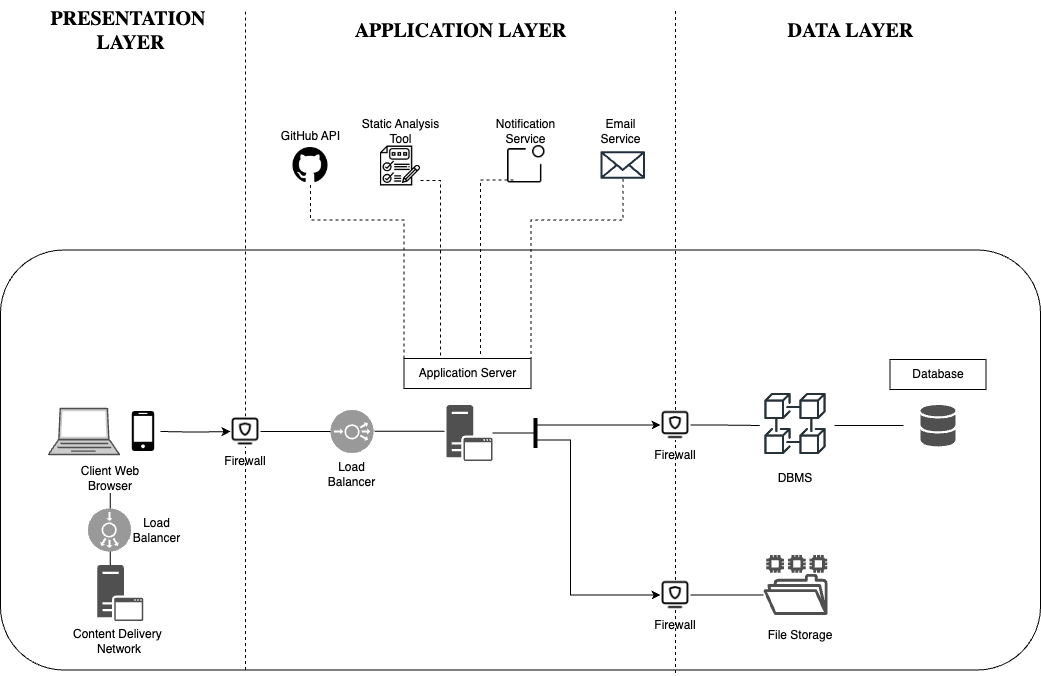
\includegraphics[scale=0.25]{Images/DD-highlevel-architecture.drawio.png}
    \caption{High-Level Architecture of the System}
\end{figure}

\newpage 
\subsection{Component View}

\begin{figure}[H]
    \centering
    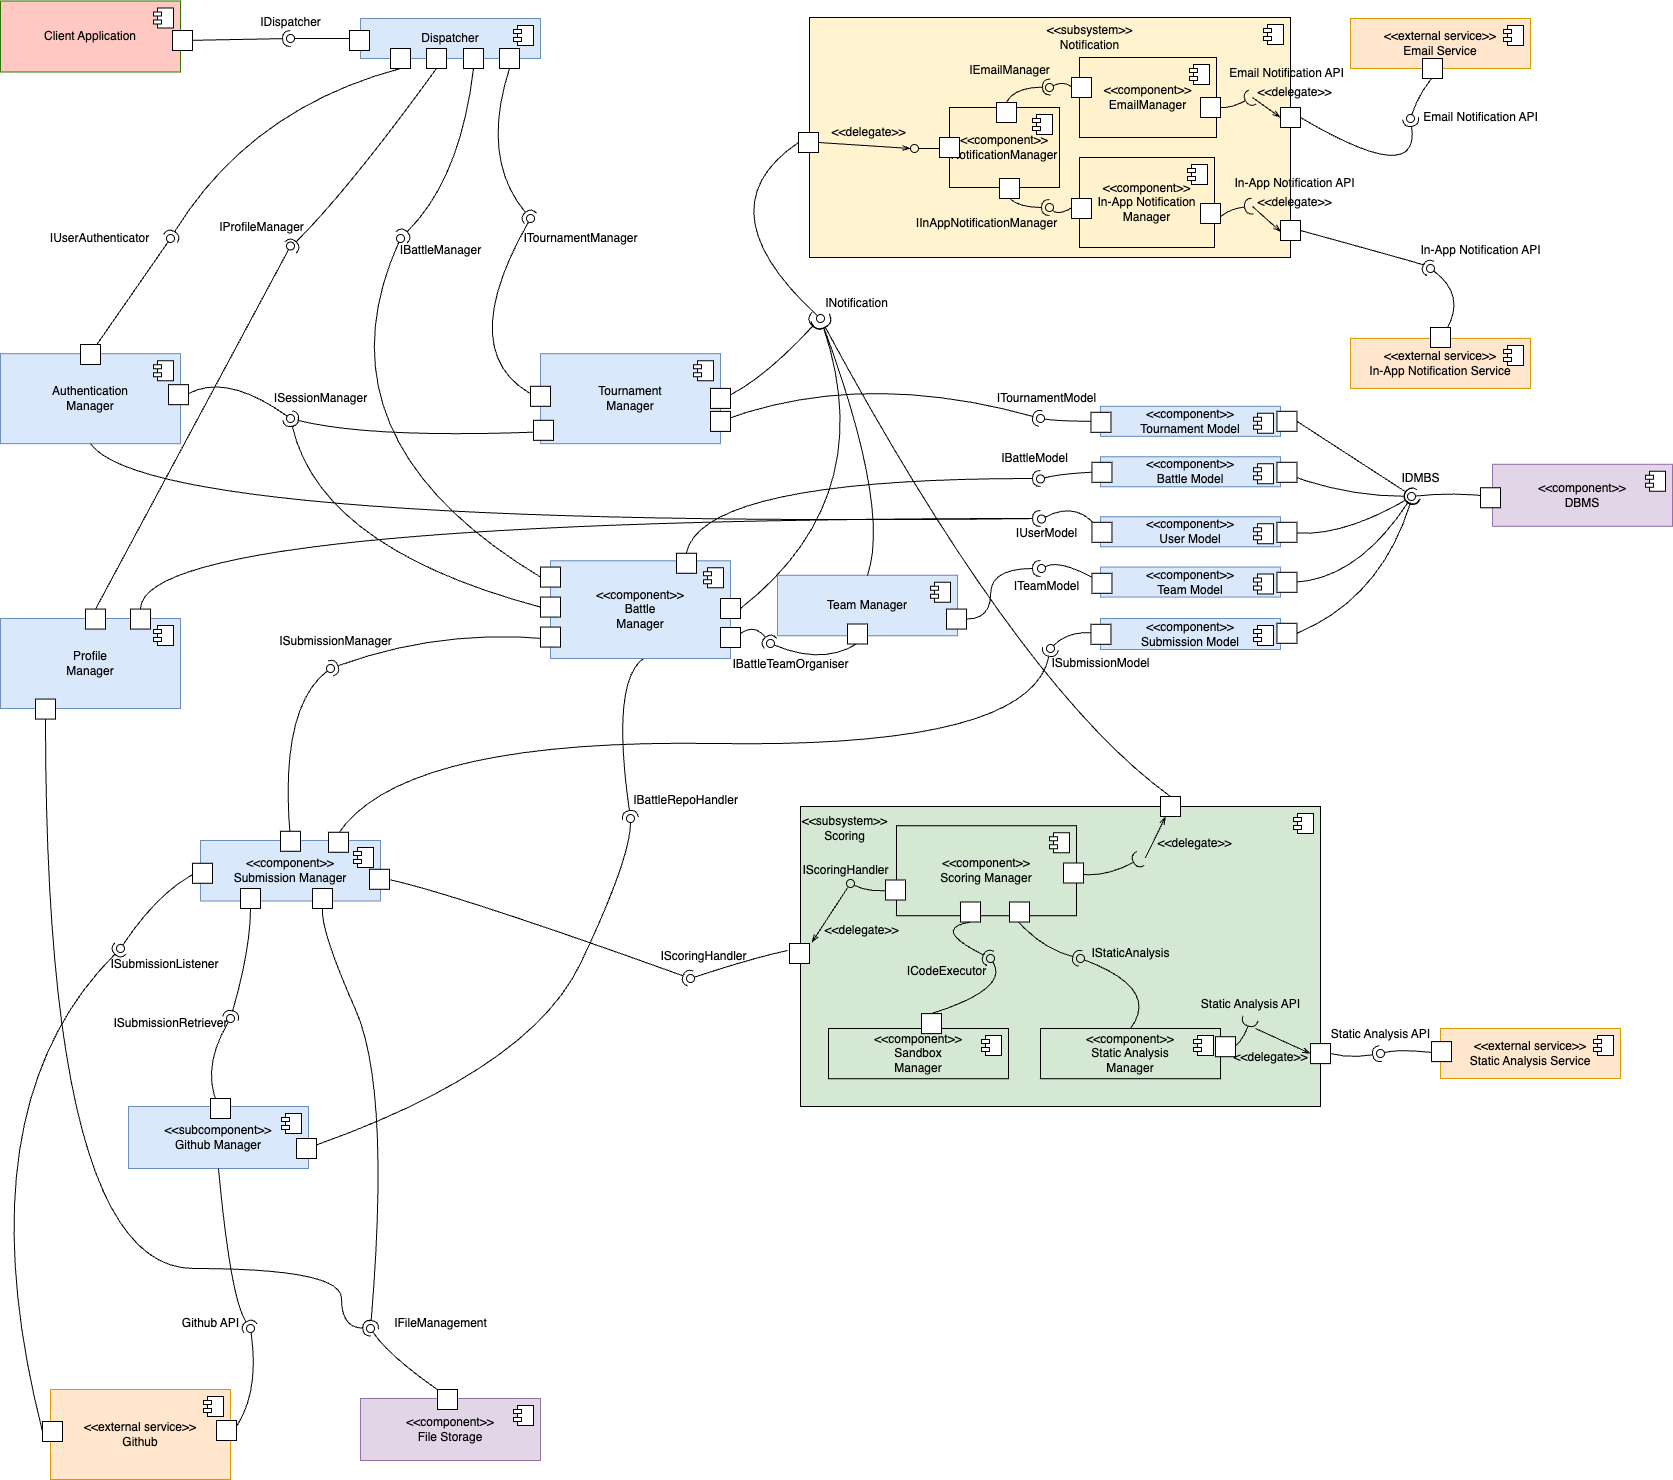
\includegraphics[width=\linewidth]{Images/DD-component.drawio.png}
    \caption{Component Diagram}
\end{figure}



\newpage
\subsection{Deployment View}
Our architecture mainly consists of 3 parts:  A Static Web Server, Application Server and Database Server.
\\
\indent Users can interact with website via a browser and a device that has browser support such as a computer, a mobile phone etc. Content Delivery Network is used for the web server which behaves as an entry point to users. It hosts the static and dynamic web content, such as .html, .css, .js, and image files, to users. Using Content Delivery Network has some advantages in terms of performance, reliability and security. CDNs speed up content delivery by decreasing the distance between where content is stored and where it needs to go, reducing file sizes to increase load speed, optimizing server infrastructure to respond to user requests more quickly. Also  if a server, a data center, or an entire region of data centers goes down, CDNs can still deliver content from other servers in the network. Moreover, it is also very useful from the security perspective. With their many servers, CDNs are better able to absorb large amounts of traffic, even unnatural traffic spikes from a DDoS attack, than a single origin server.
\\
\indent Then we have our Application Server which is hosted on the cloud with 2-4 instances. Also we have an additional Static Analysis Server.
\\
\indent At the Data Layer, we have database servers which includes database and DBMS with a firewall. 


\begin{figure}[H]
    \centering
    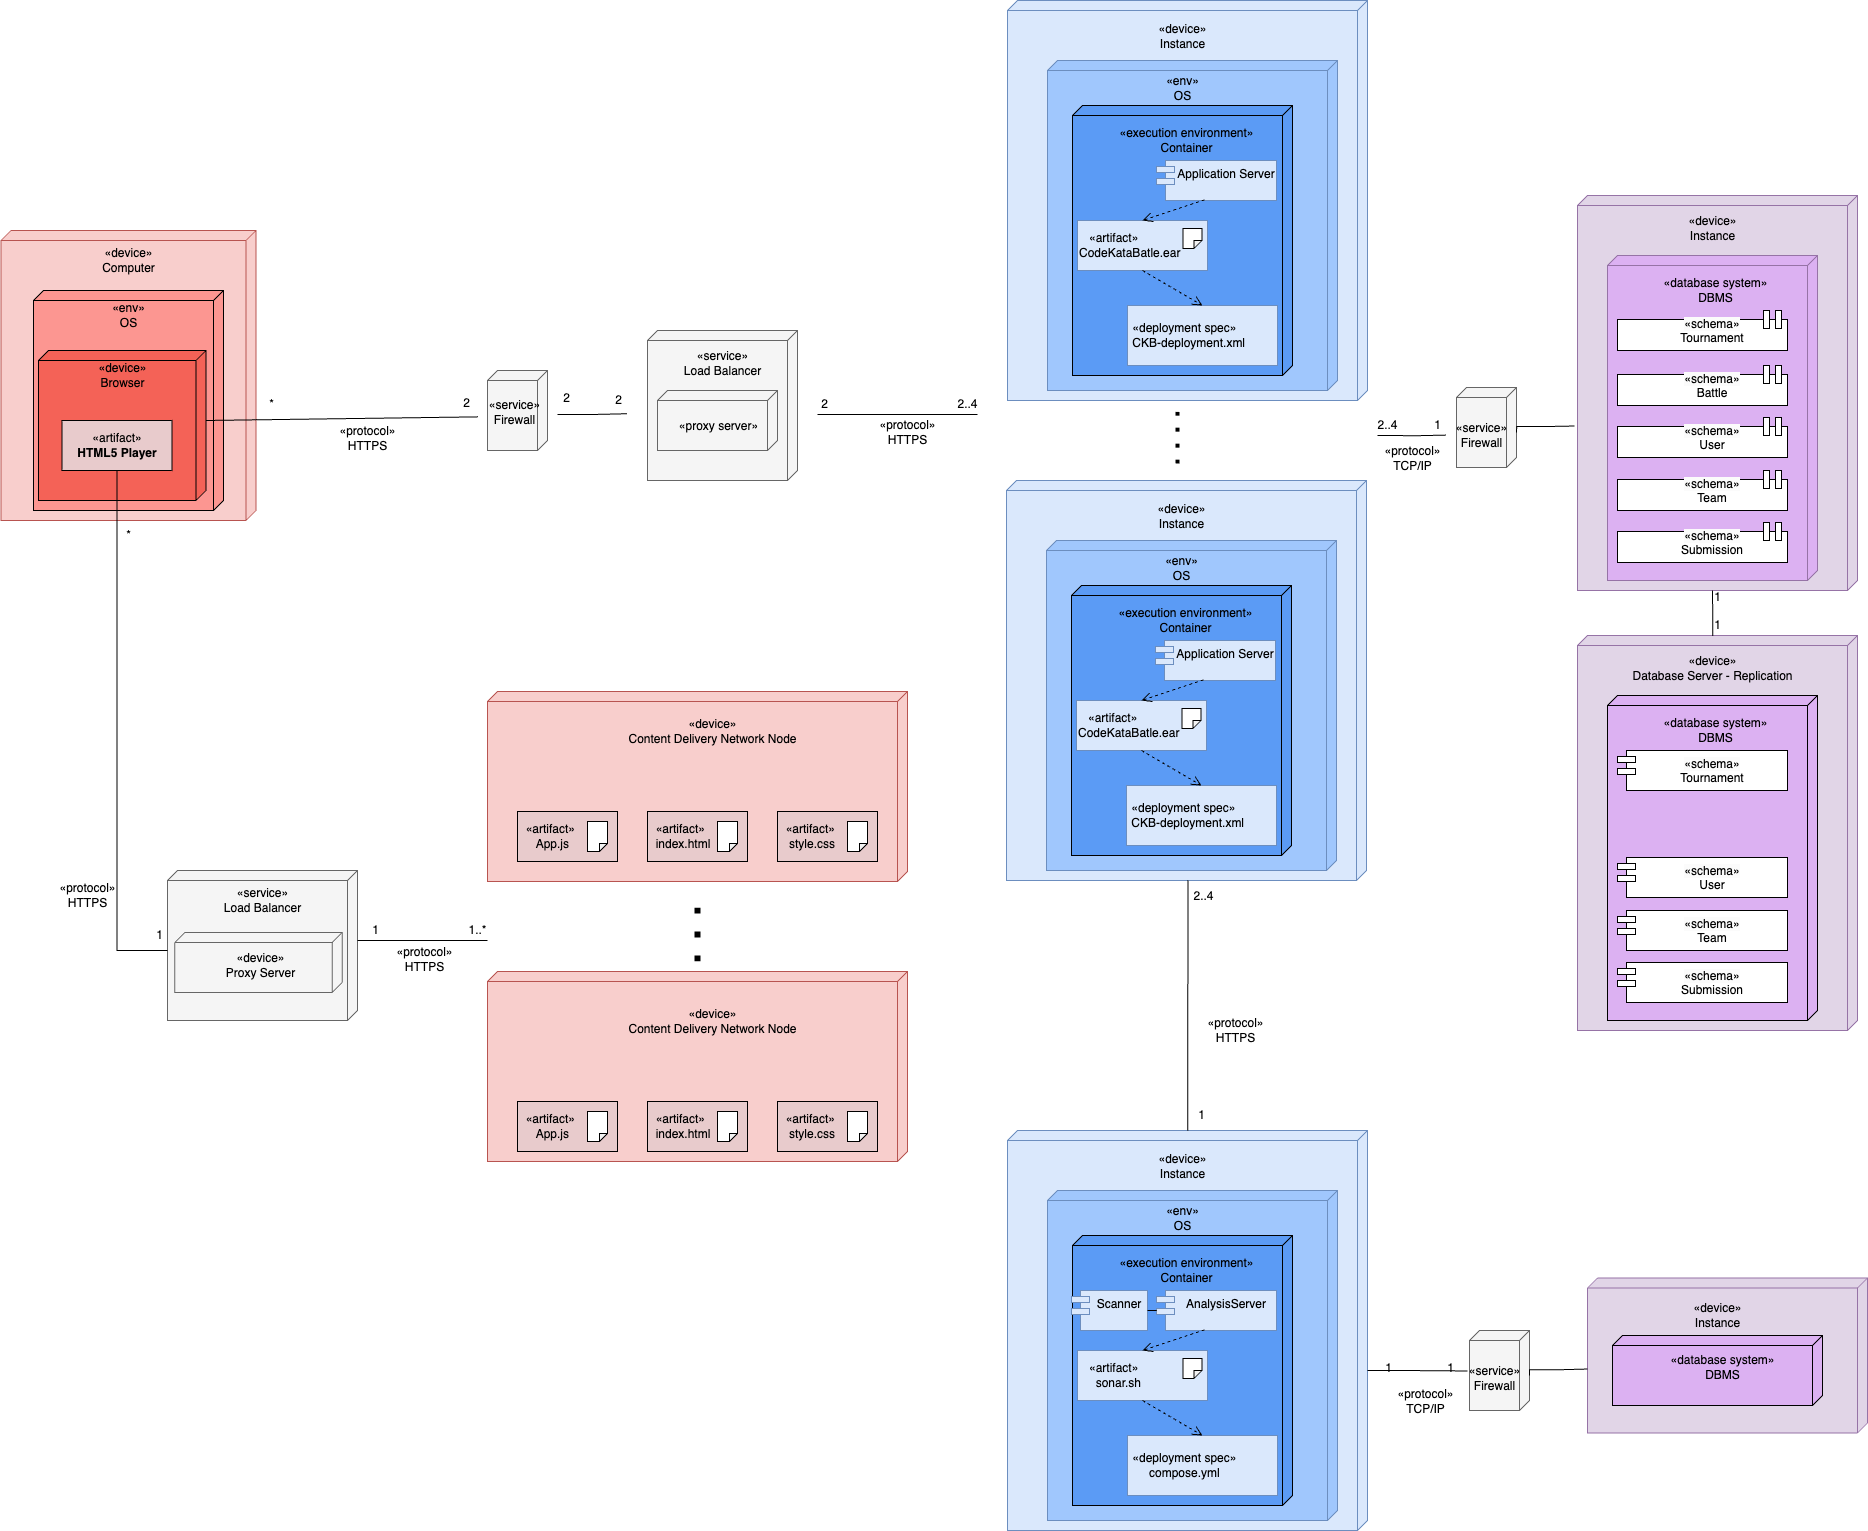
\includegraphics[scale=0.25]{Images/DD-deployment.drawio.png}
    \caption{Deployment Diagram}
\end{figure}

The deployment diagram offers a more detailed view over the hardware and software resources of the application:
\\
\indent \textbf{User Device:} User device can be any device that supports a web browser.
\\
\indent \textbf{Static Web Content:} The static web content of CodeKata Battle is hosted by Content Delivery Network with a Load Balancer distributing traffic and workload. The nodes in CDN can be scaled to very large numbers because it needs low computation power and memory. Geographically distributed nodes can be helpful to provide web interface with great performance in terms of speed. Briefly, The this content is static and all of its code is run on the
client’s machine,by browser, so there is no need for any logic to be implemented on the CDN side.
\\
\indent \textbf{Application Server:} All the business logic is handled in the Application Server which is hosted on the cloud with minimum 2 and maximum 4 instances. Obviously, these numbers can change in time but ,for an initial design, using 2-4 server instances would be adequate. Also 2 load balancer is used to distributing workload among application server instances. This is the bottleneck of the application so we decided to use 2 of them. 
\indent \textbf{Static Analysis Server:} Also, our static analysis solution requires a server that is responsible for static analysis. We conclude to add a server for this solution because most of the \textbf{Static Analysis Service Providers} works in that way. We followed the \textbf{SonarQube Documentation} as a solution  \hyperlink{https://docs.sonarsource.com/sonarqube/9.9/setup-and-upgrade/install-the-server/}{\textbf{Docs}}. We strongly suggest to use of this service. The internal components described in \textbf{Component View} can change if developers decide to implement a solution with another service.
\\
\indent Distributing incoming requests among multiple servers hosted on the cloud can helps us to fulfill some technical constraints:
\\
\indent \textbf{Reliability}: Cloud providers often offer high reliability through redundant resources and infrastructure. If one server fails, others can take over, minimizing downtime. Regular backups and disaster recovery options further enhance reliability.

\indent \textbf{Availability}: High availability is a key feature of these kind of hosting. Multiple instances in the cloud use multiple data centers around the world, ensuring that your services remain accessible even during local outages or disruptions.

\indent \textbf{Security}: Cloud providers invest heavily in security measures, including physical security of data centers, network security, and data encryption. Monitoring tools and firewall helps to sustain a secure application server.

\indent \textbf{Scalability}: Increasing or decreasing the size and amount of the instances can help to deal with changing request loads that servers have to respond to, also with the help of load balancing. Because of the changes in traffic or workload, we would need different computation and memory capacity. You can easily scale your server resources up or down based on demand, ensuring optimal performance without overpaying for unused capacity.

\indent \textbf{Maintainability}: Cloud providers handle hardware maintenance, updates, and patches, allowing us to focus on core business and application development. Also logging and monitoring tools generally works well with this kind of hosting other than in-house hosting or custom solutions we can develop.

\indent \textbf{Portability}: Cloud environments support portability and interoperability. You can move applications and data across different cloud environments or providers with relative ease, avoiding vendor lock-in and allowing for flexibility in deployment choices.
\\
\indent \textbf{Database}: This instance contains database with necessary schemas and database managements system. It is used with a replication It is also has a replicated version of itself, because of our \textbf{reliability} and \textbf{availability} constraints. By replicating data across multiple nodes or locations, the system can ensure high \textbf{availability}. If one node fails, the others can continue to operate, minimizing downtime and ensuring continuous access to data. Also, in the event of a major failure or disaster affecting the primary data center, having replicas ensures that data is not lost and can be quickly recovered. Also our static analysis solution requires a database instance for analysis server which is independent from other database instances.
\\
\indent \textbf{Firewalls:} Firewall services act as a security gatekeeper for a system's business and data layers, screening incoming connections. They enhance security by enforcing rules that either permit or block traffic, safeguarding the system from illicit access or harmful attacks.

\indent \textbf{Load Balancers:} A load balancer is employed to evenly distribute incoming traffic across various instances of an application. This strategy optimizes the use of resources, boosts performance, and maintains high availability. By doing so, the load balancer aids in managing a significant influx of requests, preventing the application from being overwhelmed or suffering downtime, and contributes to overall stability.


\newpage
\subsection{Runtime View}
This section includes the interaction of components for the important functionalities of the system. 
\subsubsection{User Registration}
Firstly, user sends the registration form from the registration screen. The pages differs for students and educators (see $UI_{1}$). Then system check that if this email exists or not. If it does not exis, the system creates user and send verification to user email. After verification, user registration process is completed successfully.
\begin{figure}[H]
    \centering
    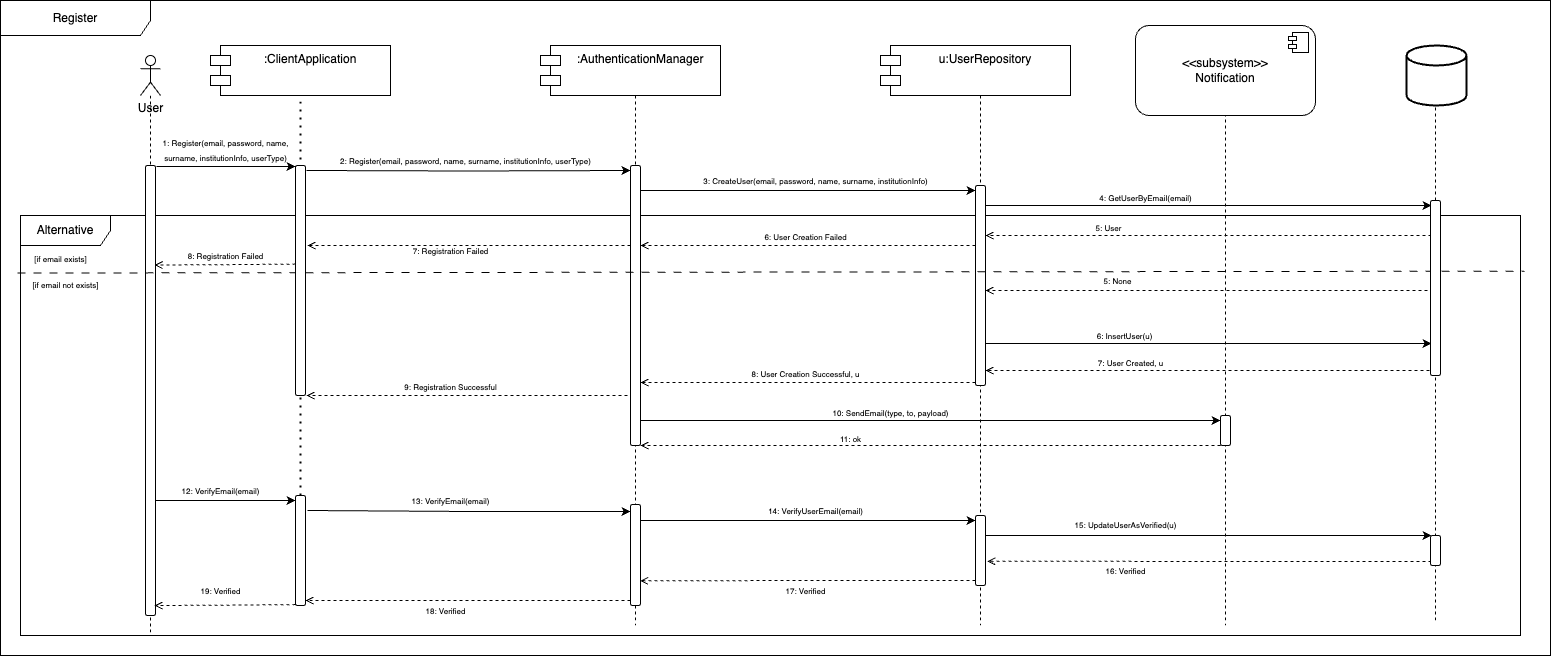
\includegraphics[width=\linewidth]{Images/runtime/register_runtime.drawio.png}
    \caption{$RW_{1}$} Registration
\end{figure}

\subsubsection{User Login}
Students and educators both need to login in order to use system functionalities. Only authenticated users can see the tournaments, battle etc. So user enters the credentials and system responds with respect to correctness of credentials.
\begin{figure}[H]
    \centering
    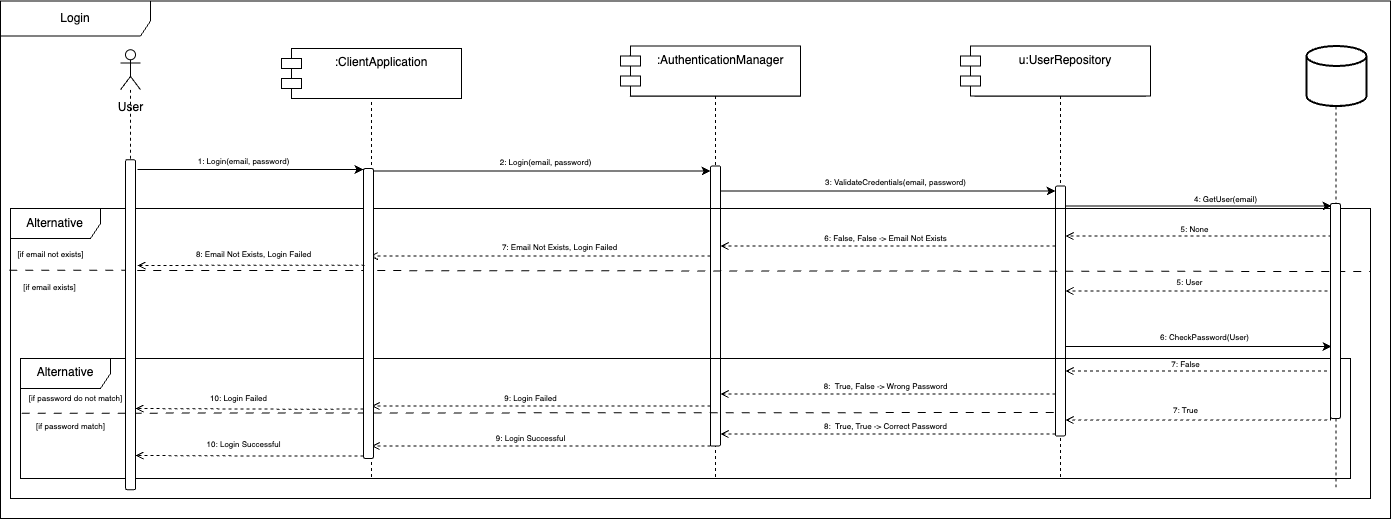
\includegraphics[width=\linewidth]{Images/runtime/login_runtime.drawio.png}
    \caption{$RW_{2}$} Login
\end{figure}

\subsubsection{View Tournament}
In this view some alternative ways to see the tournaments are shown. Fundamentally, students and educator can see all the tournaments. Also some options are available to filter the tournaments. After listing list of tournaments user can select and view on from them.
\begin{figure}[H]
    \centering
    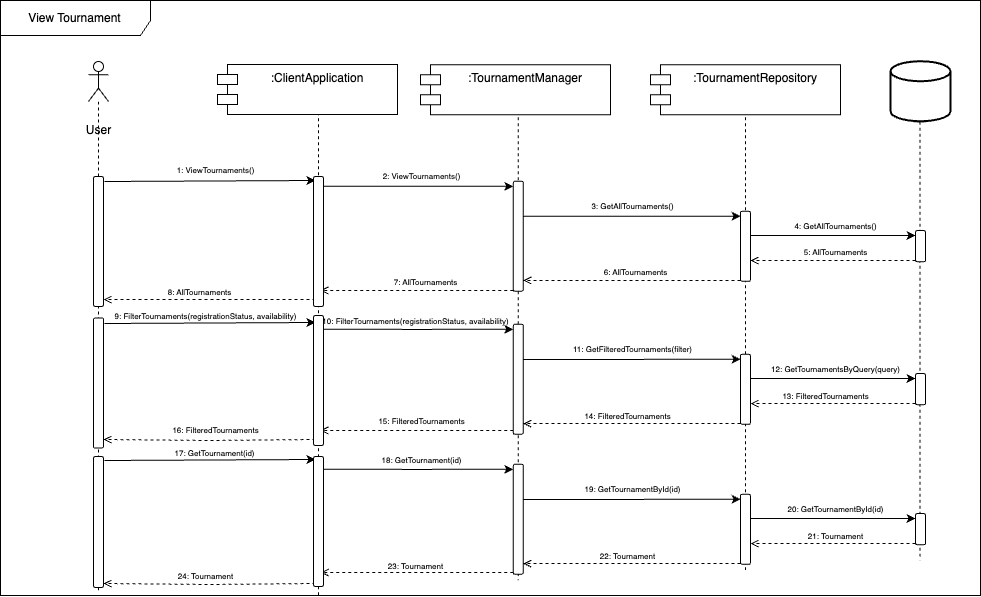
\includegraphics[width=\linewidth]{Images/runtime/view_tournament_runtime.drawio.png}
    \caption{$RW_{3}$} View Tournament
\end{figure}

\subsubsection{View Template}
This runtime view is a demonstration of all view functions of the application. Thanks to our layered approach, we can view the entities such as tournaments, battles, profiles. Consider this runtime view as a template.
\begin{figure}[H]
    \centering
    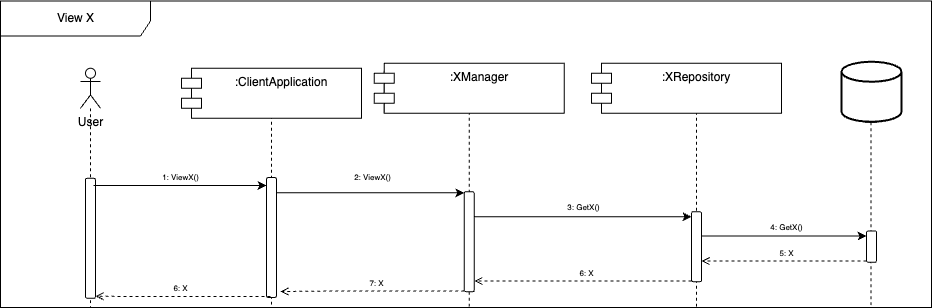
\includegraphics[width=\linewidth]{Images/runtime/view_template_runtime.drawio.png}
    \caption{$RW_{4}$} View Entity Template
\end{figure}

\subsubsection{Edit Profile}
This runtime view explains the sequences when a user want to edit their profiles. In the repository level there are functions for user type specific but this logic is encapsulated by Profile Manager, so endpoint is way simple.
\begin{figure}[H]
    \centering
    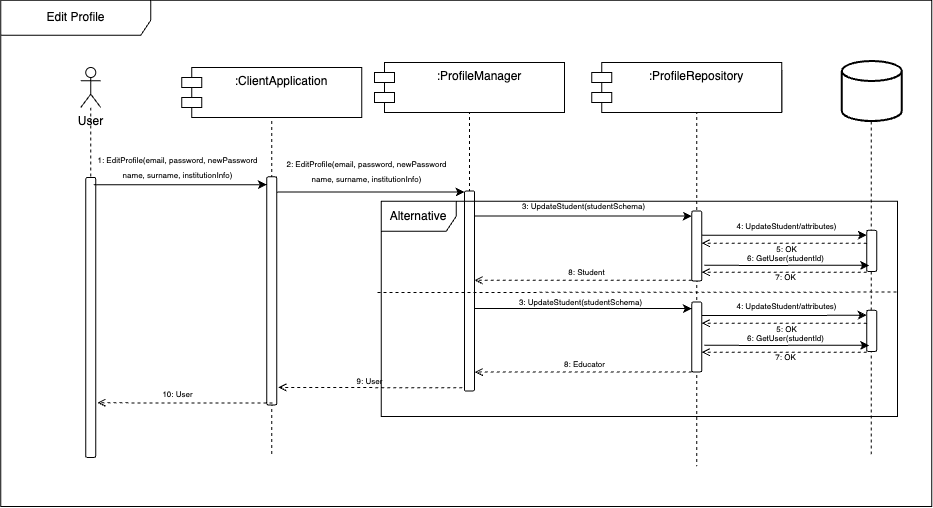
\includegraphics[width=\linewidth]{Images/runtime/edit_profile.drawio.png}
    \caption{$RW_{5}$} Edit Profile
\end{figure}


\subsubsection{Notification Subsystem}
Notification Subsystem is one of the core parts of the application. It consists of multiple components however other components of application sees only few function provided by Notification Manager. In this diagram we show a notification that send both email and in app notification. In other diagram we do not show all the process about notification, just show trigger function and response. This diagram explain what happens in a detailed way when a notification is sent .
\begin{figure}[H]
    \centering
    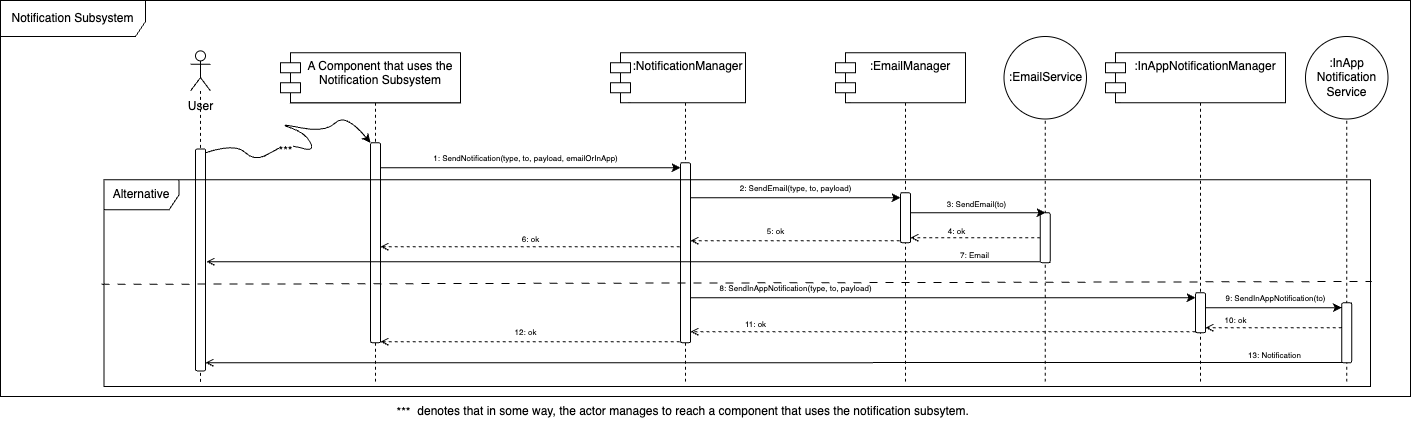
\includegraphics[width=\linewidth]{Images/runtime/notification_runtime.drawio.png}
    \caption{$RW_{6}$} Notification Subsystem
\end{figure}

\subsubsection{Session Management}
The main components that provides endpoints uses session information. They use the functions provided by ISesssionManager to retrieve user from the token provided in endpoint. 
\begin{figure}[H]
    \centering
    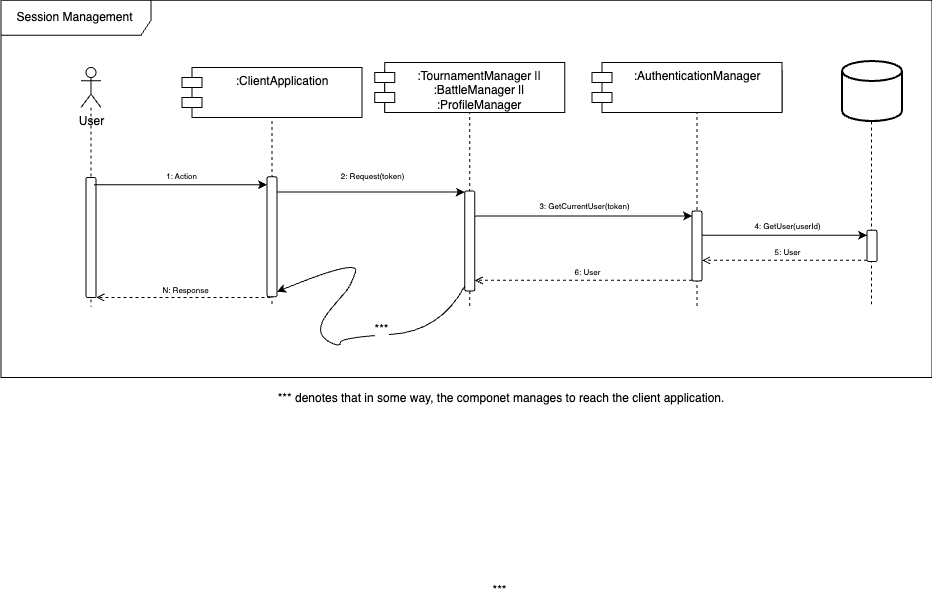
\includegraphics[width=\linewidth]{Images/runtime/session_runtime.drawio.png}
    \caption{$RW_{7}$} Session Management
\end{figure}


\subsubsection{Inspect Submission}
Educators can need to inspect a submission to view them or score manually.  This diagram explains the steps starting from battle to manual scoring. Of course manual scoring can be done if it is enabled in that battle.
\begin{figure}[H]
    \centering
    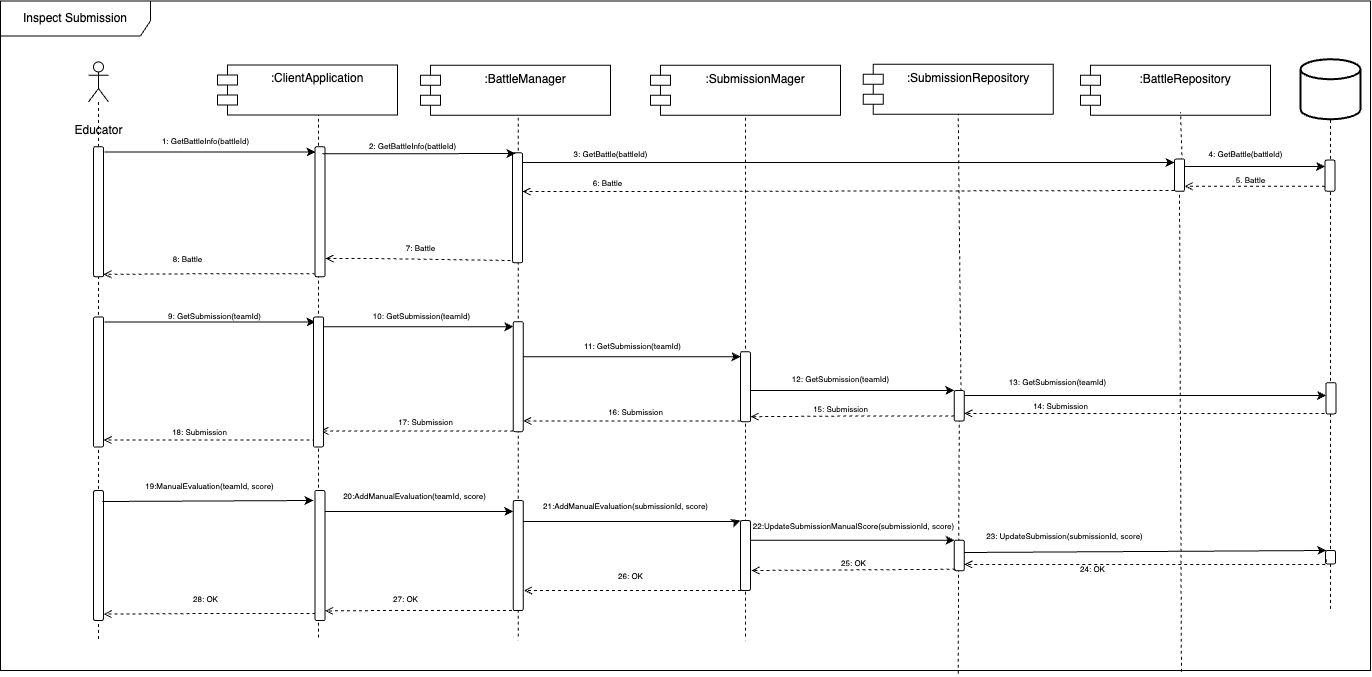
\includegraphics[width=\linewidth]{Images/runtime/inspect_submission_runtime.drawio.png}
    \caption{$RW_{8}$} Inspect Submission
\end{figure}


\subsubsection{Register To Tournament}
Students can register to Tournament. This diagram shows this process in a sequential way.
\begin{figure}[H]
    \centering
    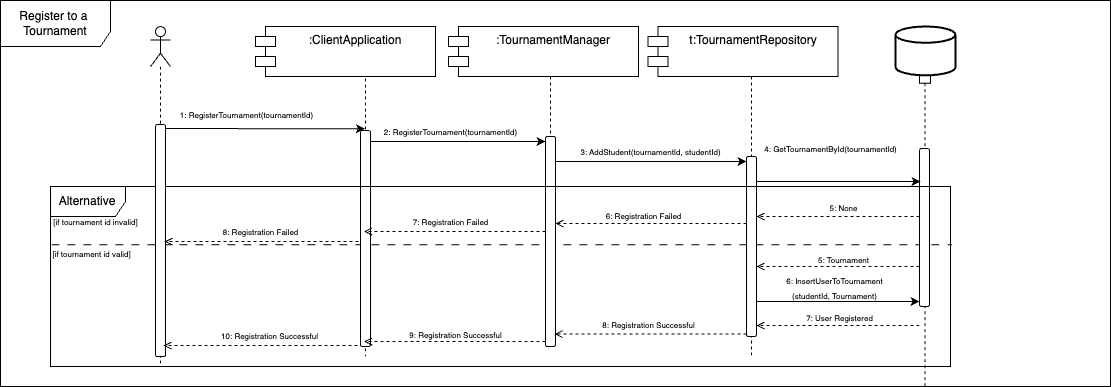
\includegraphics[width=\linewidth]{Images/runtime/register_tournament_runtime.drawio.png}
    \caption{$RW_{9}$} Register to Tournament
\end{figure}


\subsubsection{Register To Battle}
Students can register to Battle. This diagram shows this process in a sequential way.
\begin{figure}[H]
    \centering
    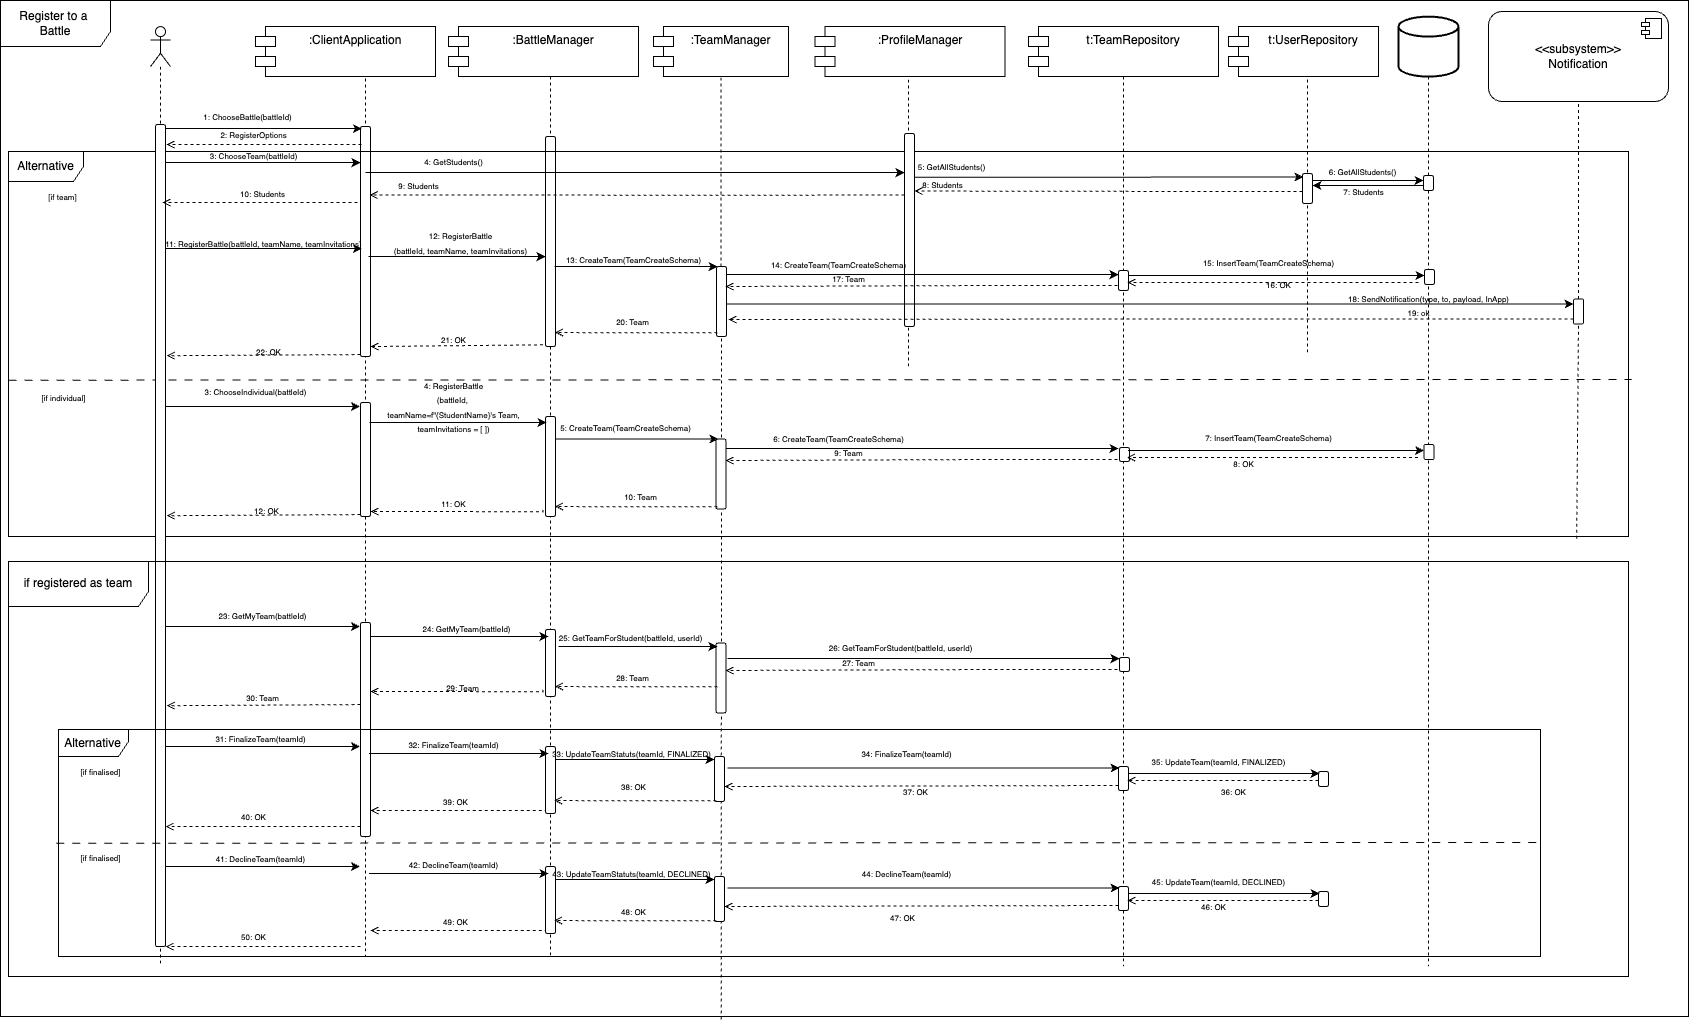
\includegraphics[width=\linewidth]{Images/runtime/register_battle_runtime.drawio.png}
    \caption{$RW_{10}$} Register to Battle
\end{figure}

\subsubsection{Create Tournament}
Educators can create tournaments. After tournament creation notifications are sent to all users.
\begin{figure}[H]
    \centering
    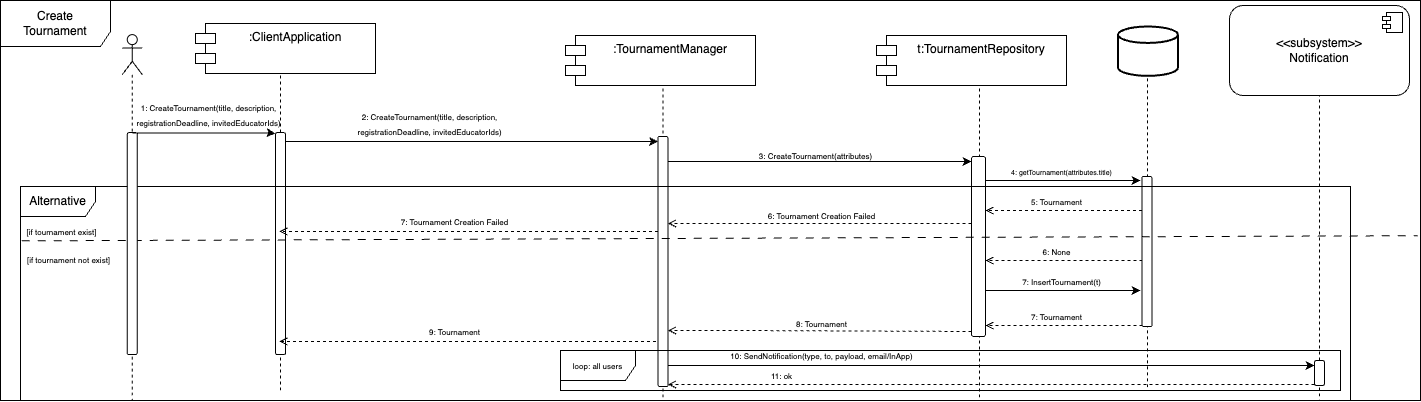
\includegraphics[width=\linewidth]{Images/runtime/create_tournament_runtime.drawio.png}
    \caption{$RW_{11}$} Create Tournament
\end{figure}

\subsubsection{Create Battle}
Educators can create battles. After battle creation notifications are sent to all users in tournament.
\begin{figure}[H]
    \centering
    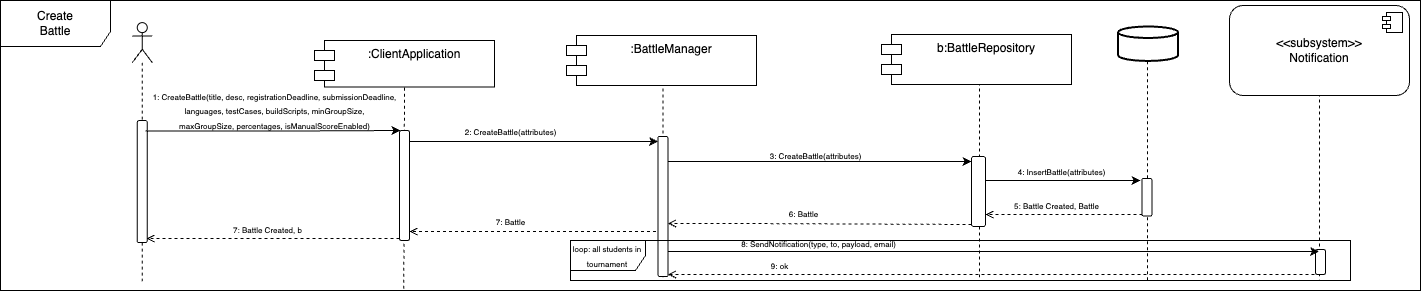
\includegraphics[width=\linewidth]{Images/runtime/create_battle_runtime.drawio.png}
    \caption{$RW_{12}$} Create Battle
\end{figure}

\subsubsection{Submission Handling}
This diagram shows the sequential actions when a submission occurs. Submission Handling is triggered by the Github commit from students.
\begin{figure}[H]
    \centering
    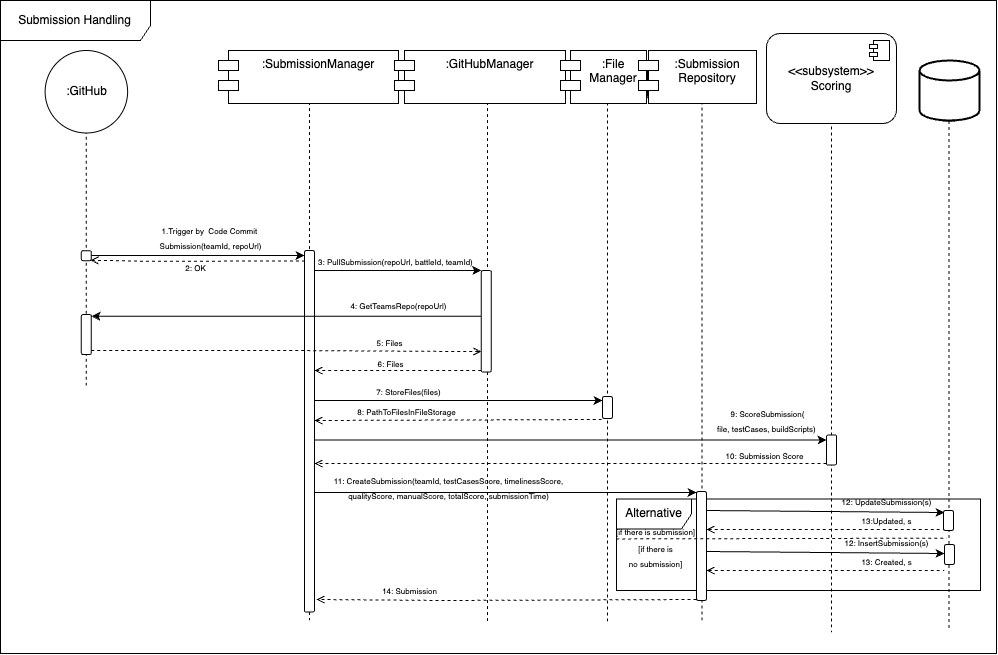
\includegraphics[width=\linewidth]{Images/runtime/submission_handling_runtime.drawio.png}
    \caption{$RW_{13}$} Submission Handling
\end{figure}



\subsubsection{Scoring Subsystem}
This diagram shows the sequential actions in scoring subsystem. Similar to notification subsystem, it has another components inside and only gives simple methods to other components in order to calculate scores.
\begin{figure}[H]
    \centering
    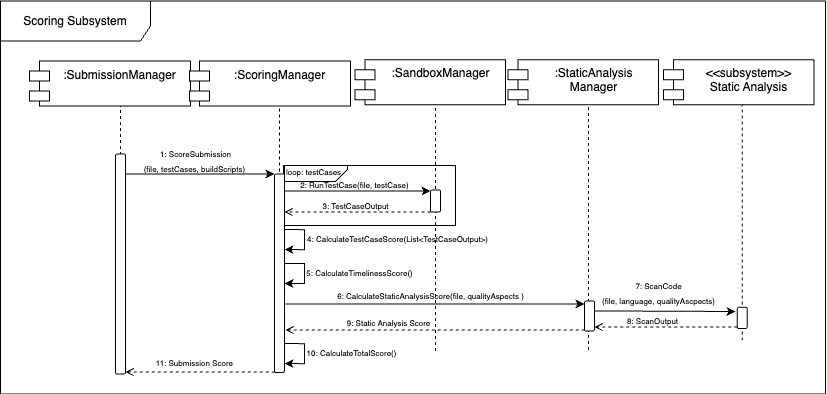
\includegraphics[width=\linewidth]{Images/runtime/scoring_subsystem_runtime.drawio.png}
    \caption{$RW_{14}$} Scoring Subsystem
\end{figure}



\subsubsection{Static Analysis Subsystem}
This diagram shows the sequential actions during static analysis. The Web API used by Scanner is not shown here because it is used for setup for authentication. Also API provides some endpoint to control server instead of CLI operations.
\begin{figure}[H]
    \centering
    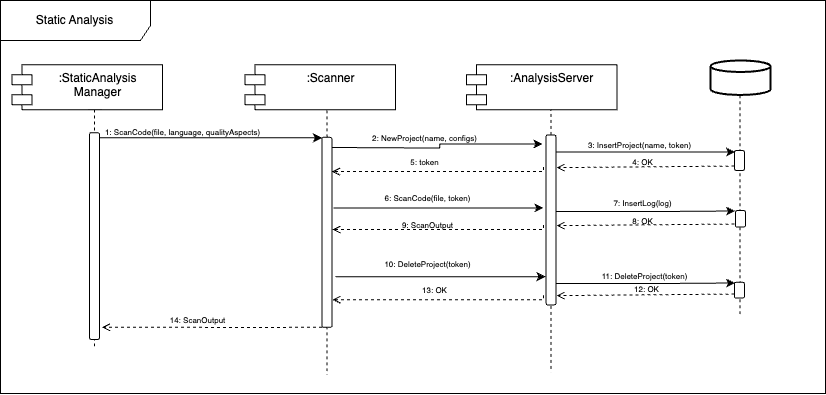
\includegraphics[width=\linewidth]{Images/runtime/static_analysis.drawio.png}
    \caption{$RW_{15}$} Static Analysis Subsystem
\end{figure}

\subsubsection{Battle Github Repository Creation}
After battle registration deadlines passed a Github repository must be created to be used by students. This diagram explains the Github repository creation of the battle.
\begin{figure}[H]
    \centering
    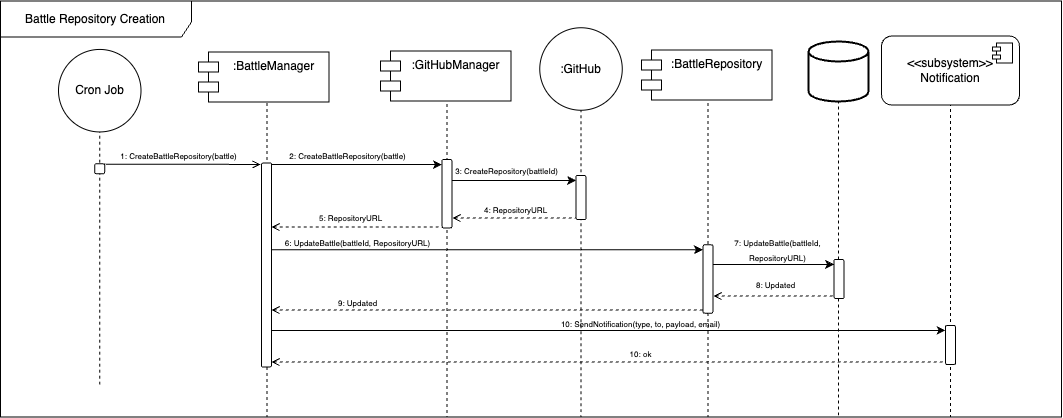
\includegraphics[width=\linewidth]{Images/runtime/battle_repository_runtime.drawio.png}
    \caption{$RW_{16}$} Battle Github Repository Creation
\end{figure}

\subsection{Component Interfaces}
In this section, we explain the interfaces and provided methods and returned objects. Also a class diagram is provided to show the dependencies and relations between the interfaces. Also at the end of the section endpoints provided by the system is listed and explained.

The Class Diagram is the same as Domain Level Class Diagram in RASD except some additional schmeas to demonstrate the data structures used in interfaces.
\begin{figure}[H]
    \centering
    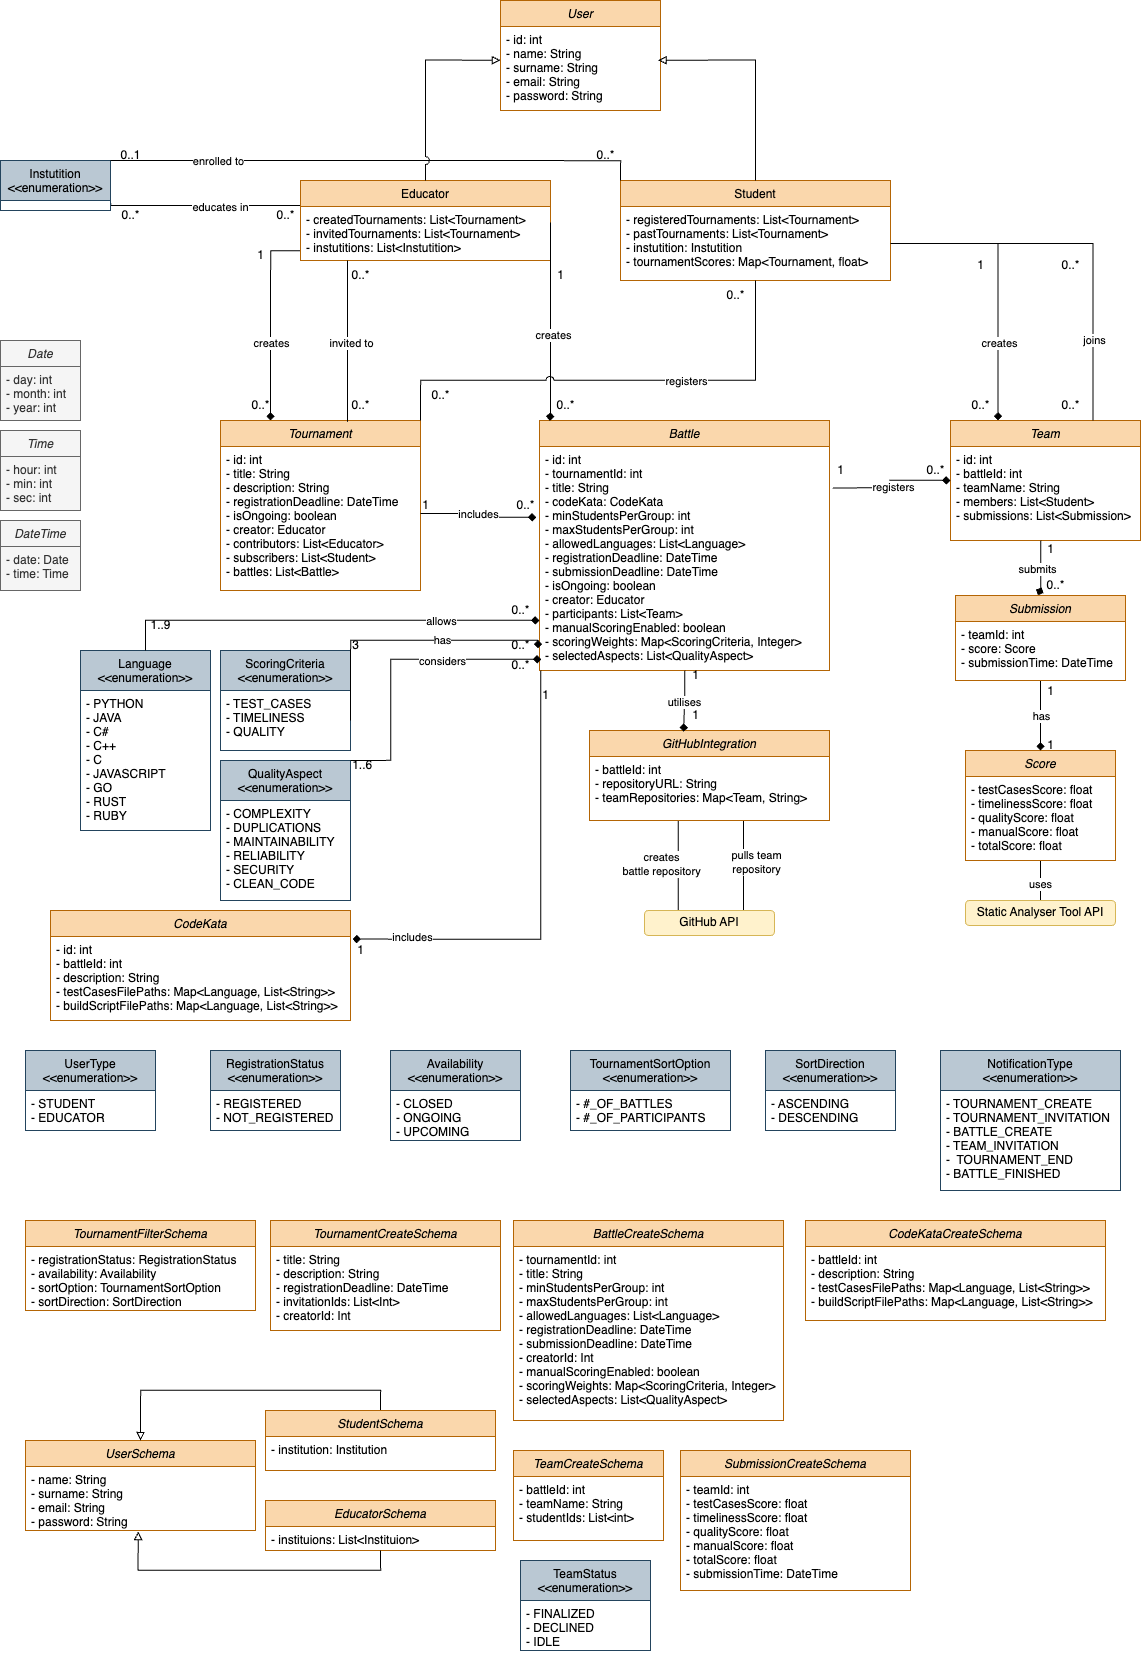
\includegraphics[width=\linewidth]{Images/DD-Class Diagram.drawio.png}
    \caption{Class Diagram (Based on RASD)}
\end{figure}

\subsubsection{IUserAuthenticator}
This Interface contains endpoints related to authentication of users. Endpoints explained in a detailed way at the end of the section. Just signatures are available here.
\begin{itemize}
\item Register(email: String, password: String, name: String, surname: String, institutionInfo: List<Institution>, userType: UserType) -> HTTP Response
\item Login(email: String, password: String) -> HTTP Response
\item Logout()-> HTTP Response
\item VerifyEmail(email:String) -> HTTP Response
\end{itemize}

\subsubsection{IProfileManager}
This Interface contains endpoints related to profiles of users. Endpoints explained in a detailed way at the end of the section. Just signatures are available here.
\begin{itemize}
\item GetMyProfile() -> HTTP Response
\item GetProfile(userId: int) -> HTTP Response
\item EditProfile(email: String, password: String, newPassword: String, name: String, surname: String, institutionInfo: List<Institution>) -> HTTP Response
\item GetEducators()-> HTTP Response
\item GetStudents()-> HTTP Response
\end{itemize}
\subsubsection{ITournamentManager}
This Interface contains endpoints related to Tournament. Endpoints explained in a detailed way at the end of the section. Just signatures are available here.
\begin{itemize}
\item GetTournaments(registrationStatus: RegistrationStatus, availability: Availability, sortOption: TournamentSortOption, sortDirection: SortDirection) -> HTTP Response
\item GetTournamentInfo(tournamentId: int) -> HTTP Status
\item RegisterTournament(tournamentId: int) -> HTTP Status
\item GetTournamentBattles(tournamentId: int, minGroupSize: int, maxGroupSize: int, startDate: DateTime, endDate: DateTime, registrationStatus: RegistrationStatus, institution: Institution, languages: List<Language>, educatorIds: List<int>, searchText: String) -> HTTP Response
\item GetTournamentLeaderboard(tournamentId: int) -> HTTP Response
\item ExportTournamentLeaderboard(tournamentId: int) -> HTTP Response
\item CreateTournament(title: String, description: String, registrationDeadline: DateTime, invitedEducatorIds: List<int>) -> HTTP Response
\item AnswerTournamentInvitation(tournamentId: int, isAccepted: boolean, educatorId: int) -> HTTP Response
\item EndTournament(tournamentId: int) -> HTTP Response
\end{itemize}

\subsubsection{IBattleManager}
This Interface contains endpoints related to Battle. Endpoints explained in a detailed way at the end of the section. Just signatures are available here.
\begin{itemize}
\item GetBattleInfo(battleId: int) -> HTTP Response
\item GetSubmission(teamId: int) -> HTTP Response
\item GetBattleRankings(battleId: int) -> HTTP Response
\item RegisterBattle(battleId: int, teamName: String, teamInvitations: List<int>) -> HTTP Response 
\item AnswerBattleInvitation(teamId: int, isAccepted: boolean, studentId: int) -> HTTP Response
\item FinalizeTeam(teamId: int) -> HTTP Response
\item DeclineTeam(teamId: int) -> HTTP Response
\item GetTeam(teamId: int) -> HTTP Response
\item GetMyTeam(battleId: int) -> HTTP Response
\item GetTeamScore(teamId: int) -> HTTP Response
\item AddManualEvaluation(teamId: int, score: float) -> HTTP Response
\item CreateBattle(title: String, description: String, registrationDeadline: DateTime, submissionDeadline: DateTime, languages: List<Language>, testCases: Map<String, List<File> >, buildScripts: Map<String, File>, minGroupSize: int, maxGroupSize: int, percentages: Map<String, int>, isManualScoreEnabled: boolean) -> HTTP Response 
\item ExportBattleLeaderboard(battleId: int) -> HTTP Response
\end{itemize}

\subsubsection{ISessionManager}
This Interface provides session related methods to components. Other components such as \textbf{Tournament Manager}, \textbf{Battle Manager} etc. They use to retrieve current user from token provided in request header in order to apply business logic related to specific user attributes.
\begin{itemize}
    \item getCurrentUser(token: String) -> User
\end{itemize}
\subsubsection{INotification}
This Interface provides methods that enables other components to send notifications via email or in-app notifications. \textbf{INotification} abstracts the internal operations related to using notification services and provides simple methods.

\begin{itemize}
    \item SendNotification(to: String, type: NotificationType, payload: Map<String,String>, emailOrInApp: ['EMAIL', 'NOTIFICATION']) -> boolean \\
    Calls methods below
    \item sendEmail(to: String, type: NotificationType, payload: Map<String,String>) -> boolean \\ This method sends email to given email with predefined email type related to a template and payload of it. Same method exists in \textbf{IEmailManager}.
    \item sendInAppNotification(userId: int, type: NotificationType, payload: Map<String,String>) -> boolean \\ This method sends in-app notification to given user id with predefined notification type related to a template and payload of it.Same method exists in \textbf{IInAppNotificationManager}.
\end{itemize}
\subsubsection{Repository Interfaces}
These interfaces are mainly responsible for the query management and communication with DBMS. They provide database query methods for other components. 
\begin{enumerate}
    \item \textbf{Tournament Repository}
    \begin{itemize}
        \item GetAllTournaments() -> List<Tournament> 
        \item GetFilteredTournament(filter: TournamentFilterSchema) -> List<Tournament>\\
        \item GetTournamentById(tournamentId: int) -> Tournament
        \item CreateTournament(attributes: TournamentCreateSchema) -> int (Tournament Id)
        \item EndTournament(tournamentId: int) -> boolean
        \item AddEducator(tournamentId: int, educatorId: int) -> boolean
        \item AddStudent(tournamentId: int, studentId: int) -> boolean
    \end{itemize}  
    \item \textbf{Battle Repository}
    \begin{itemize}
        \item GetBattle(battleId: int) -> Battle
        \item CreateBattle(attributes: BattleCreateSchema) -> Battle
        \item UpdateBattle(battleId: int, repoUrl: String) -> boolean
        \item CreateCodeKata(attributes: CodeKataCreateSchema) -> int (CodeKata Id)
    \end{itemize}
    \item \textbf{User Repository}
    \begin{itemize}
        \item CreateUser() -> User (This is a abstract method, use CreateStudent or CreateEducator)
        \item CreateStudent(attributes: StudentSchema) -> Student
        \item CreateEducator(attributes: EducatorSchema) -> Educator
        \item GetUser(userId: int) -> User
        \item GetAllStudents() -> List<User>
        \item GetAllEducators() -> List<User>
        \item UpdateStudent(attributes: StudentSchema) -> Student
        \item UpdateEducator(attributes: EducatorSchema) -> Educator
        \item DeleteUser(userId: int) -> boolean
        \item VerifyUserEmail(email:String) -> boolean
        \item ValidateCredentials(email: String, password: String) -> boolean, boolean
    \end{itemize}
    \item \textbf{Team Repository}
    \begin{itemize}
        \item CreateTeam(attributes: TeamCreateSchema) -> Team 
        \item FinalizeTeam(teamId: int) -> boolean
        \item DeclineTeam(teamId: int) -> boolean
        \item UpdateStudentStatus(teamId: int, studentId: int, isAccepted: boolean) -> boolean
        \item GetTeam(teamId: int) -> Team
        \item GetTeamForStudent(battleId: int, userId: int) -> Team
    \end{itemize}
    \item \textbf{Submission Repository}
    \begin{itemize}
        \item CreateSubmission(attributes: SubmissionCreateSchema) -> Submission \\
        This function overwrites the existing submission, more precisely, safe deletes it.
        \item GetSubmission(teamId: int) -> Submission
        \item GetSubmissions(battleId: int) -> List<Submission>
        \item UpdateSubmissionManualScore(submissionId: int, score: float) -> boolean
    \end{itemize}
\end{enumerate}
\subsubsection{IBattleTeamOrganiser}
\begin{itemize}
    \item UpdateTeamStatus(teamId: int, status: TeamStatus) -> boolean
    \item CreateTeam(attributes: TeamCreateSchema) -> Team
    \item GetTeam(teamId: int) -> Team
    \item GetTeamForStudent(battleId: int, studentId: int) -> Team
    \item AcceptTeamInvitation(teamId: int, studentId: int) -> boolean
    \item DeclineTeamInvitation(teamId: int, studentId: int) -> boolean
\end{itemize}
\subsubsection{ISubmissionManager}
\begin{enumerate}
    \item GetSubmission(teamId: int) -> Submission
    \item GetBattleScores(battle: Battle) -> List<Map<Team, int> >
   \item AddManualEvaluation(submissionId: int, score: float) -> boolean
\end{enumerate}
\subsubsection{ISubmissionListener}
\begin{enumerate}
    \item Submission(teamId: int, repoUrl: string) -> HTTP Status \\
    This is an endpoint responsible to be triggered by Github Actions Workflow created by teams. When they made a new commit, they  send a request to this endpoint.
\end{enumerate}
\subsubsection{ISubmissionRetriever}
\begin{enumerate}
    \item PullSubmission(repoUrl: String, battleId: int, teamId: int) -> String \\
    This method provides the url of a folder in the file storage system. The pulled repository content is stored in this folder with a naming using battleId and teamId. The component using this method is then responsible for other actions.
    \end{enumerate}
\subsubsection{IScoringHandler}
\begin{enumerate}
   \item ScoreSubmission(code: File, testCaseFiles: Map<Language, List<File> >, buildScripts: Map<Language, List<File> >) -> float
  \item CalculateTestCaseScore(List<TestCaseOutput>) -> float
   \item CalculateStaticAnalysisScore(code: File, qualityAspects: List<QualityAspect>) -> float
   \item CalculateTimelinessScore(submissionDate: DateTime, battleStartDate: DateTime) -> float
   \item \textbf{ICodeExecutor}
   \begin{itemize}
        \item CreateSandboxEnviroment(language: Language, build
       \item RunTestCase(code: File, language: Language, testCase: File) -> TestCaseOutput (custom schema contains logs and test case result)
   \end{itemize}
   \item \textbf{IStaticAnalysis}
   \begin{itemize}
       \item CalculateStaticAnalysisScore(codeUrls: List<String>, language: Language, qualityAspects: List<QualityAspect>) -> float
   \end{itemize}
\end{enumerate}
\subsubsection{IBattleRepoHandler}
\begin{itemize}
    \item CreateBattleRepository(battle: Battle) -> String (Repository URL)
\end{itemize}
\subsubsection{IFileManagement}
\item StoreFiles(files: List<File> ) -> List<String> (Path to Files)
\item FetchFiles(url: String) -> File
\subsubsection{IScanner}
\item ScanCode(file: File, language: Language, qualityAspects: List<QualityAspect>)) -> ScanOutput
\item \textbf{IAnalysisServer}
\begin{itemize}
    \item NewProject(name: String, configs: Map) -> String
    \item ScanCode(file: File, token: String) -> ScanOutput (**complex response, look service provider documentation for further exploration)
    \item DeleteProject(token: String) -> boolean
\end{itemize}
\item \textbf{Web API}
This is API provided by external service to manage the server and other operations such as authentication etc. At first no specific use other than authentication, but it is a good practice to manage server with API instead of CLI commands and bash scripts in long term.
\subsubsection{IGithubAPI}
This is the external API used to retrieve submission from Github. This Interface is explained later.
\subsubsection{File Storage API}
This is the external service to store and manager files stored in the application. Cloud Object Storage is used. This Interface is explained later.

\subsubsection{API Endpoints}
\begin{enumerate}
    \item \textbf{Endpoint Auth/Register} \\
    \textbf{Method:} POST \\
    Request Body:\\
    \begin{itemize}
        \item email: String
        \item password: String
        \item name: String
        \item surname: String
        \item institutionInfo: List<Institution>
        \item userType: UserType
    \end{itemize}
    Response:\\
    \begin{itemize}
        \item \textbf{200} \\
        \begin{itemize}
            \item message: "User is registered successfully"
            \item id: int
        \end{itemize}
                \item \textbf{400} \\
        \begin{itemize}
            \item message: "Email exists"
        \end{itemize}
    \end{itemize}
    \item \textbf{Endpoint Auth/Login} \\
    \textbf{Method:} POST \\
    Request Body:\\
    \begin{itemize}
        \item email: String
        \item password: String
    \end{itemize}
    Response:\\
    \begin{itemize}
        \item \textbf{200} \\
        \begin{itemize}
            \item message: "User is logged in successfully"
            \item token: String
        \end{itemize}
                \item \textbf{400} \\
        \begin{itemize}
            \item message: "Credentials are wrong"
        \end{itemize}
    \end{itemize}
    \item \textbf{Endpoint Auth/Logout} \\
    \textbf{Method:} POST \\
    Header:\\
    \begin{itemize}
        \item token: String
    \end{itemize}
    Response:\\
    \begin{itemize}
        \item \textbf{200} \\
        \begin{itemize}
            \item message: "User is logged out successfully"
        \end{itemize}
                \item \textbf{400} \\
        \begin{itemize}
            \item message: "Something went wrong"
        \end{itemize}
    \end{itemize}
    \item \textbf{Endpoint Auth/VerifyEmail} \\
    \textbf{Method:} POST \\
    Request Body:\\
    \begin{itemize}
        \item email: String
    \end{itemize}
    Response:\\
    \begin{itemize}
        \item \textbf{200} \\
        \begin{itemize}
            \item message: "User is verified successfully"
        \end{itemize}
                \item \textbf{400} \\
        \begin{itemize}
            \item message: "Something went wrong"
        \end{itemize}
    \end{itemize}
    \item \textbf{Endpoint Profile/GetMyProfile} \\
    \textbf{Method:} GET \\
    Header:\\
    \begin{itemize}
        \item token: String
    \end{itemize}
    Response:\\
    \begin{itemize}
        \item \textbf{200} \\
        \begin{itemize}
            \item profile: Student
        \end{itemize}
        \item \textbf{200} \\
        \begin{itemize}
            \item profile: Educator
        \end{itemize}
        \item \textbf{400} \\
        \begin{itemize}
            \item message: "Something went wrong"
        \end{itemize}
    \end{itemize}
    \item \textbf{Endpoint Profile/GetProfile/:userId} \\
    \textbf{Method:} GET \\
    Header:\\
    \begin{itemize}
        \item token: String
    \end{itemize}
    Response:\\
    \begin{itemize}
        \item \textbf{200} \\
        \begin{itemize}
            \item profile: Student
        \end{itemize}
        \item \textbf{200} \\
        \begin{itemize}
            \item profile: Educator
        \end{itemize}
        \item \textbf{400} \\
        \begin{itemize}
            \item message: "Something went wrong"
        \end{itemize}
    \end{itemize}
    \item \textbf{Endpoint Profile/EditProfile} \\
    \textbf{Method:} POST \\
    Header:\\
    \begin{itemize}
        \item token: String
    \end{itemize}
    Request Body: \\
    \begin{itemize}
        \item email: String
        \item password: String
        \item newPassword: String
        \item name: String
        \item surname: String
        \item institutionInfo: List<Institution>
    \end{itemize}
    Response:\\
    \begin{itemize}
        \item \textbf{200} \\
        \begin{itemize}
            \item profile: Student
        \end{itemize}
        \item \textbf{200} \\
        \begin{itemize}
            \item profile: Educator
        \end{itemize}
        \item \textbf{400} \\
        \begin{itemize}
            \item message: "Email exists"
        \end{itemize}
        \item \textbf{400} \\
        \begin{itemize}
            \item message: "Password is wrong"
        \end{itemize}
    \end{itemize}
    \item \textbf{Endpoint Profile/GetEducators} \\
    \textbf{Method:} GET \\
    Header:\\
    \begin{itemize}
        \item token: String
    \end{itemize}
    Response:\\
    \begin{itemize}
        \item \textbf{200} \\
        \begin{itemize}
            \item educators: List<Educator>
        \end{itemize}
        \item \textbf{400} \\
        \begin{itemize}
            \item message: "Something went wrong"
        \end{itemize}
    \end{itemize}
        \item \textbf{Endpoint Profile/GetStudents} \\
    \textbf{Method:} GET \\
    Header:\\
    \begin{itemize}
        \item token: String
    \end{itemize}
    Response:\\
    \begin{itemize}
        \item \textbf{200} \\
        \begin{itemize}
            \item students: List<Student>
        \end{itemize}
        \item \textbf{400} \\
        \begin{itemize}
            \item message: "Something went wrong"
        \end{itemize}
    \end{itemize}
    \item \textbf{Endpoint Tournament/GetTournaments} \\
    \textbf{Method:} GET \\
    Header:\\
    \begin{itemize}
        \item token: String
    \end{itemize}
    Request Parameters: \\
    \begin{itemize}
        \item registrationStatus: RegistrationStatus
        \item availability: Availability
        \item sortOption: TournamentSortOption
        \item sortDirection: SortDirection
    \end{itemize}
    Response:\\
    \begin{itemize}
        \item \textbf{200} \\
        \begin{itemize}
            \item tournaments: List<Tournament>
        \end{itemize}
        \item \textbf{400} \\
        \begin{itemize}
            \item message: "Something went wrong"
        \end{itemize}
    \end{itemize}
    \item \textbf{Endpoint Tournament/GetTournamentInfo/:tournamentId} \\
    \textbf{Method:} GET \\
    Header:\\
    \begin{itemize}
        \item token: String
    \end{itemize}
    Response:\\
    \begin{itemize}
        \item \textbf{200} \\
        \begin{itemize}
            \item tournament: Tournament
        \end{itemize}
        \item \textbf{400} \\
        \begin{itemize}
            \item message: "Something went wrong"
        \end{itemize}
    \end{itemize}
    \item \textbf{Endpoint Tournament/RegisterTournament/:tournamentId} \\
    \textbf{Method:} POST \\
    Header:\\
    \begin{itemize}
        \item token: String
    \end{itemize}
    Response:\\
    \begin{itemize}
        \item \textbf{200} \\
        \begin{itemize}
            \item tournamentId: int
        \end{itemize}
        \item \textbf{400} \\
        \begin{itemize}
            \item message: "Can not register Tournament"
        \end{itemize}
    \end{itemize}
    \item \textbf{Endpoint Tournament/GetTournamentBattles/:tournamentId} \\
    \textbf{Method:} GET \\
    Header:\\
    \begin{itemize}
        \item token: String
    \end{itemize}
    Request Parameters:\\
    \begin{itemize}
        \item minGroupSize: int
        \item maxGroupSize: int
        \item startDate: DateTime
        \item endDate: DateTime
        \item registrationStatus: RegistrationStatus
        \item institution: Instituion
        \item langauges: List<Language>
        \item educatorIds: List<int>
        \item searchText: String
    \end{itemize}
    Response:\\
    \begin{itemize}
        \item \textbf{200} \\
        \begin{itemize}
            \item battles: List<Battle>
        \end{itemize}
        \item \textbf{400} \\
        \begin{itemize}
            \item message: "Something went wrong"
        \end{itemize}
    \end{itemize}
    \item \textbf{Endpoint Tournament/GetTournamentLeaderboard/:tournamentId} \\
    \textbf{Method:} GET \\
    Header:\\
    \begin{itemize}
        \item token: String
    \end{itemize}
    Response:\\
    \begin{itemize}
        \item \textbf{200} \\
        \begin{itemize}
            \item leaderboard: List<Map<String, int> >
        \end{itemize}
        \item \textbf{400} \\
        \begin{itemize}
            \item message: "Something went wrong"
        \end{itemize}
    \end{itemize}
    \item \textbf{Endpoint Tournament/ExportTournamentRankings/:tournamentId} \\
    \textbf{Method:} GET \\
    Header:\\
    \begin{itemize}
        \item token: String
    \end{itemize}
    Response:\\
    \begin{itemize}
        \item \textbf{200} \\
        \begin{itemize}
            \item leaderboard: StreamResponse(File)
        \end{itemize}
        \item \textbf{400} \\
        \begin{itemize}
            \item message: "Something went wrong"
        \end{itemize}
    \end{itemize}
    \item \textbf{Endpoint Tournament/CreateTournament} \\
    \textbf{Method:} POST \\
    Header:\\
    \begin{itemize}
        \item token: String
    \end{itemize}
    Request Body:\\
    \begin{itemize}
        \item title: String
        \item description: String
        \item registrationDeadline: DateTime
        \item invitedEducatorIds: List<int>
    \end{itemize}
    Response:\\
    \begin{itemize}
        \item \textbf{200} \\
        \begin{itemize}
            \item tournament: Tournament
        \end{itemize}
        \item \textbf{400} \\
        \begin{itemize}
            \item message: "Tournament can not be created"
        \end{itemize}
    \end{itemize}
    \item \textbf{Endpoint Tournament/AnswerTournament/:tournamentId} \\
    \textbf{Method:} POST \\
    Header:\\
    \begin{itemize}
        \item token: String
    \end{itemize}
    Request Body:\\
    \begin{itemize}
        \item isAccepted: boolean
        \item educatorId: int
    \end{itemize}
    Response:\\
    \begin{itemize}
        \item \textbf{200} \\
        \begin{itemize}
            \item message: "Tournament invitation is answered"
        \end{itemize}
        \item \textbf{400} \\
        \begin{itemize}
            \item message: "Something went wrong"
        \end{itemize}
    \end{itemize}
    \item \textbf{Endpoint Tournament/EndTournament/:tournamentId} \\
    \textbf{Method:} POST \\
    Header:\\
    \begin{itemize}
        \item token: String
    \end{itemize}
    Response:\\
    \begin{itemize}
        \item \textbf{200} \\
        \begin{itemize}
            \item message: "Tournament is ended"
        \end{itemize}
        \item \textbf{400} \\
        \begin{itemize}
            \item message: "Something went wrong"
        \end{itemize}
    \end{itemize}
    \item \textbf{Endpoint Battle/GetBattleInfo/:battleId} \\
    \textbf{Method:} GET \\
    Header:\\
    \begin{itemize}
        \item token: String
    \end{itemize}
    Response:\\
    \begin{itemize}
        \item \textbf{200} \\
        \begin{itemize}
            \item battle: Battle
        \end{itemize}
        \item \textbf{400} \\
        \begin{itemize}
            \item message: "Something went wrong"
        \end{itemize}
    \end{itemize}
    \item \textbf{Endpoint Battle/GetBattleRankings/:battleId} \\
    \textbf{Method:} GET \\
    Header:\\
    \begin{itemize}
        \item token: String
    \end{itemize}
    Response:\\
    \begin{itemize}
        \item \textbf{200} \\
        \begin{itemize}
            \item rankings: List<Map<String, int> >
        \end{itemize}
        \item \textbf{400} \\
        \begin{itemize}
            \item message: "Something went wrong"
        \end{itemize}
    \end{itemize}
    \item \textbf{Endpoint Battle/RegisterBattle/:battleId} \\
    \textbf{Method:} POST \\
    Header:\\
    \begin{itemize}
        \item token: String
    \end{itemize}
    Request Body:\\
    \begin{itemize}
        \item teamName: String
        \item teamInvitations: List<int>
    \end{itemize}
    Response:\\
    \begin{itemize}
        \item \textbf{200} \\
        \begin{itemize}
            \item message: "Registered successfully"
        \end{itemize}
        \item \textbf{400} \\
        \begin{itemize}
            \item message: "Something went wrong"
        \end{itemize}
    \end{itemize}
    \item \textbf{Endpoint Battle/AnswerBattleInvitation/:teamId} \\
    \textbf{Method:} POST \\
    Header:\\
    \begin{itemize}
        \item token: String
    \end{itemize}
    Request Body:\\
    \begin{itemize}
        \item isAccepted: boolean
        \item studentId: int
    \end{itemize}
    Response:\\
    \begin{itemize}
        \item \textbf{200} \\
        \begin{itemize}
            \item message: "Battle invitation is answered"
        \end{itemize}
        \item \textbf{400} \\
        \begin{itemize}
            \item message: "Something went wrong"
        \end{itemize}
    \end{itemize}
    \item \textbf{Endpoint Battle/FinalizeTeam/:teamId} \\
    \textbf{Method:} POST \\
    Header:\\
    \begin{itemize}
        \item token: String
    \end{itemize}
    Response:\\
    \begin{itemize}
        \item \textbf{200} \\
        \begin{itemize}
            \item message: "Team is finalized"
        \end{itemize}
        \item \textbf{400} \\
        \begin{itemize}
            \item message: "Something went wrong"
        \end{itemize}
    \end{itemize}
    \item \textbf{Endpoint Battle/DeclineTeam/:teamId} \\
    \textbf{Method:} POST \\
    Header:\\
    \begin{itemize}
        \item token: String
    \end{itemize}
    Response:\\
    \begin{itemize}
        \item \textbf{200} \\
        \begin{itemize}
            \item message: "Team is declined"
        \end{itemize}
        \item \textbf{400} \\
        \begin{itemize}
            \item message: "Something went wrong"
        \end{itemize}
    \end{itemize}
    \item \textbf{Endpoint Battle/GetTeam/:teamId} \\
    \textbf{Method:} GET \\
    Header:\\
    \begin{itemize}
        \item token: String
    \end{itemize}
    Response:\\
    \begin{itemize}
        \item \textbf{200} \\
        \begin{itemize}
            \item team: Team
        \end{itemize}
        \item \textbf{400} \\
        \begin{itemize}
            \item message: "Something went wrong"
        \end{itemize}
    \end{itemize}
    \item \textbf{Endpoint Battle/GetMyTeam/:battleID} \\
    \textbf{Method:} GET \\
    Header:\\
    \begin{itemize}
        \item token: String
    \end{itemize}
    Response:\\
    \begin{itemize}
        \item \textbf{200} \\
        \begin{itemize}
            \item team: Team
        \end{itemize}
        \item \textbf{400} \\
        \begin{itemize}
            \item message: "You don't have a team for this battle"
        \end{itemize}
    \end{itemize}
    \item \textbf{Endpoint Battle/GetTeamScore/:teamId} \\
    \textbf{Method:} GET \\
    Header:\\
    \begin{itemize}
        \item token: String
    \end{itemize}
    Response:\\
    \begin{itemize}
        \item \textbf{200} \\
        \begin{itemize}
            \item score: Map<ScoringCriteria, int>
        \end{itemize}
        \item \textbf{400} \\
        \begin{itemize}
            \item message: "Something went wrong"
        \end{itemize}
    \end{itemize}
    \item \textbf{Endpoint Battle/AddManualEveluation/:teamId} \\
    \textbf{Method:} POST \\
    Header:\\
    \begin{itemize}
        \item token: String
    \end{itemize}
    Request Body:\\
    \begin{itemize}
        \item score: float
    \end{itemize}
    Response:\\
    \begin{itemize}
        \item \textbf{200} \\
        \begin{itemize}
            \item message: "Manual evaluation is done successfully"
        \end{itemize}
        \item \textbf{400} \\
        \begin{itemize}
            \item message: "Something went wrong"
        \end{itemize}
    \end{itemize}
     \item \textbf{Endpoint Battle/CreateBattle} \\
    \textbf{Method:} POST \\
    Header:\\
    \begin{itemize}
        \item token: String
    \end{itemize}
    Request Body:\\
    \begin{itemize}
        \item title: String
        \item description: String
        \item registrationDeadline: DateTime
        \item submissionDeadline: DateTime
        \item languages: List<Language>
        \item testCases: Map<String, List<File> >
        \item buildScripts: Map<String, File>
        \item minGroupSize: int
        \item maxGroupSize: int
        \item percentages: Map<String, int>
        \item isManualScoreEnabled: boolean
    \end{itemize}
    Response:\\
    \begin{itemize}
        \item \textbf{200} \\
        \begin{itemize}
            \item battle: Battle
        \end{itemize}
        \item \textbf{400} \\
        \begin{itemize}
            \item message: "Battle can not be created"
        \end{itemize}
    \end{itemize}
    \item \textbf{Endpoint Battle/ExportBattleRankings/:battleId} \\
    \textbf{Method:} GET \\
    Header:\\
    \begin{itemize}
        \item token: String
    \end{itemize}
    Response:\\
    \begin{itemize}
        \item \textbf{200} \\
        \begin{itemize}
            \item rankings: StreamResponse(File)
        \end{itemize}
        \item \textbf{400} \\
        \begin{itemize}
            \item message: "Something went wrong"
        \end{itemize}
    \end{itemize}
\end{enumerate}
\newpage
\subsection{Selected Architectural Styles and Patterns}
\subsubsection{3-Tier Architecture}
The 3-Tier Architecture is a widely-used design pattern in the development of web-based applications. It divides the application architecture into three distinct layers, each with a specific function, promoting a modular and scalable approach. The three layers are:

Presentation Layer (Client Tier): This is the user interface of the application. It's responsible for displaying user interface elements and processing user input. It communicates with the Business Logic Layer for data processing and operations.

Business Logic Layer (Application Tier): This layer is the core of the application, handling the business logic. It processes user requests, performs calculations, and makes logical decisions. It communicates between the Presentation Layer and the Data Layer, acting as a mediator for data retrieval and storage.

Data Layer (Data Tier): This layer is responsible for managing the database. It stores, retrieves, and updates data in a structured format. This layer ensures data integrity and security.

Benefits of 3-Tier Architecture:

Modularity: Each layer can be developed and maintained independently. This separation of concerns makes the system more manageable and organized.

Scalability: Each layer can be scaled independently based on demand. For example, you can increase the capacity of the data layer without altering the application or presentation layers.

Flexibility and Reusability: Changes in one layer generally do not affect the other layers. For example, the UI can be redesigned without altering the business logic. Similarly, the business logic can be modified without impacting the database structure.

Improved Security: The separation allows for better security measures. For example, the data layer can be secured independently of the other layers, minimizing the risk of data breaches.

Ease of Maintenance: Individual layers can be updated or repaired without affecting the entire system.

Compared to Other Architectures:

Vs. Monolithic Architecture: A monolithic architecture combines all three tiers into a single application. It is simpler to deploy and manage but can become unwieldy as the application grows, and it lacks the modularity and scalability of 3-tier architecture.

Vs. Microservices Architecture: Microservices architecture breaks down an application into small, independently deployable services. While it offers high scalability and modularity, it is more complex in terms of inter-service communication and managing multiple small components.

In summary, the 3-tier architecture offers a balanced approach between modularity, scalability, and manageability. It is well-suited for applications where these aspects are prioritized over the simplicity of deployment and initial development ease.

\subsubsection{Layered Architecture}
From deployment perspective we have designed Application Layer as a single component, however, from software design perspective it is layered and contains more layers. The application server is divided into Endpoints/Routers, Services (Main Business Logic), and Repositories (Data Access Layer), represents a layered architecture pattern, often used in modern web applications for clear separation of concerns. \\
\begin{enumerate}
\item \textbf{Endpoints/Routers:} This layer handles HTTP requests from clients. It's responsible for receiving requests, interpreting them, and directing them to the appropriate service layer for processing. It doesn't contain business logic or data access code; its sole purpose is to route requests to the correct parts of the application. In the component Diagram interfaces provided to Client Application includes the endpoints.

\item \textbf{Services (Main Business Logic):}This is the heart of your application. The service layer contains the core business logic. It processes requests forwarded from the endpoints/routers, applies business rules, and performs operations based on these rules. This layer doesn't directly interact with the database; instead, it communicates with the repository layer to access and manipulate data. In the component Diagram, interfaces and components which is not responsible for data access or endpoints belongs to this layer.

\item \textbf{Repositories (Data Access Layer): }The repository layer abstracts the data access logic from the service layer. It provides a collection of methods for accessing and manipulating data in your database or other storage mechanisms. The repository layer's main goal is to isolate the data access logic, making the service layer agnostic of the underlying data source and storage details. Repoistory Components are shown Component Diagram.
\end{enumerate}

\textbf{Characteristics of This Architecture:}
\begin{enumerate}
\item Separation of Concerns: Each layer has a distinct responsibility. Routers handle HTTP routing, services handle business logic, and repositories manage data access. This separation makes the application more maintainable and scalable.

\item Reusability: Each layer can be reused independently. For example, the same service layer can be used with different endpoints, and repositories can be reused across different services.

\item Testability: This architecture makes it easier to test each layer independently. For instance, you can mock the repository layer when testing services.

\item Flexibility: Changing one layer has minimal impact on the other layers. For example, you can change the data access logic without affecting the business logic.

\item Scalability: Each layer can be scaled independently based on the application's needs.
\end{enumerate}

This structure aligns with the Layered Architecture pattern, also known as the n-tier architecture pattern. In web applications, it's common to have a multi-layered architecture like this, which helps in organizing code, improving maintainability, and ensuring the application can grow and evolve over time without becoming too complex or unwieldy.

In summary, this application architecture, with clear divisions between endpoints/routers, services, and repositories, is a well-organized example of a layered architecture. This approach is widely adopted in the development of scalable, maintainable, and testable web applications.

\subsubsection{Facade}
\indent \textbf{Definition:} The Facade pattern provides a unified interface to a set of interfaces in a subsystem. It defines a higher-level interface that makes the subsystem easier to use.

\textbf{Purpose:} Facade is typically used to simplify a complex subsystem or to provide a single entry point to a level of functionality. It doesn't encapsulate the subsystem but provides a simplified interface to it.

When we consider the components in our system such as  TournamentManager or BattleManager,this pattern can help us to provide simple methods like GetBattles() or GetTournaments() without going in underlying logic in the application server. Facade simplifies the usage of the Tournament or Battle in this example.

\subsubsection{Mediators}
The Mediator pattern is a behavioral design pattern in software engineering, used to reduce complex or tight coupling between components or classes. It promotes loose coupling by encapsulating the way different sets of objects interact and communicate with each other. By introducing a mediator object, all communication between different components is centralized within the mediator, instead of being spread across multiple components.
\\
When a Component needs to communicate with another, it sends a message to the Mediator instead of sending it directly to the other Component.
The Mediator receives the message and decides how to pass these messages to the appropriate Component or Components.
The Mediator might also process or transform the data before forwarding it.
\begin{itemize}
    \item \textbf{Notification Manager:} Notification Manager behaves as Mediator between internal logic of application and Notification Services used to send notification via email or in-app notification. It help us to sustain a flexibility because it is easy to adopt Notification Manager when Notification Service is changed. Otherwise, we have to change every component when solutions used for notification is changed. \textbf{Email Manager} and \textbf{In-App Notification Manager} also help to link this internal logic to external APIs.
    \item \textbf{Static Analysis Manager:} Static Analysis Manager also acts as a Mediator operating between application server and Static Analysis Tool. Without changing internal components of system, we can adopt to changes of external Static Analysis Tool by just modifying the Static Analysis Manager.
    \item \textbf{Github Manager:} Github Managers is other component acts as a Mediator between internal components and Github as an external service. It is responsible to apply logic related to Github. The changes in the Github environment and Github API do not affect the system thanks to this component. In other words, Github Manager can be easily modified according to changes related to Github without changing other components in the application.
\end{itemize}


\subsubsection{Restful API:} A RESTful API serves as a secure interface for two computer systems to share information over the internet. In the CodeKataBattle system, this API facilitates the exchange of objects and information in JSON format via HTTP.

\subsection{Other Design Decisions}
In this section we explained further Design Decisions.
\subsubsection{Static Analysis Tool}
Static Analysis Subsystem is one of the fundamental parts of the system. It is responsible to analyse the code in order to create a Quality score. Most of the services uses a server in which Static Analysis Service is installed. Our choice for this kind of service is \hyperlink{https://docs.sonarsource.com/sonarqube/latest/}{SonarQube}. We have 3 components in our \textbf{Static Analysis Subsystem}. Scanner, Analysis Server and Database for the service. These are explained well in the SonarQube Documentation. We don't want to restrict developer to use exactly this technology so this subsystem can be adjusted to another services because this kind of architecture is common in static analysis services. Also a Web API is uses for authentication and other remote controls of the service in Analysis Server. Still, SonarQube is strongly recommended.
\subsubsection{Load Balancing, Firewall and Replication}
As we mentioned before we use Load Balancer to satisfy constraints related to \textbf{Availability}. We are aiming to less downtime by distributing incoming traffic to the running instances. Moreover, using Firewall and HTTPS for all data transactions, our \textbf{Security} constraints mentioned in the RASD will be held. Finally, sustaining Database Replication improves the \textbf{Sustainability}
by backup options and recovery plans. 

\subsubsection{Sandbox Paradigm}
In CodeKataBattle, it is needed to run submitted code via some test cases. To do so, we decided to Sandboxing. The Sandboxing in software engineering refers to a secure, controlled environment where programs can be executed without affecting the host system. This environment strictly controls the resources and permissions available to the program, ensuring that any code run within the sandbox cannot interfere with the system outside of it. This concept is crucial in scenarios where untrusted or untested code needs to be executed safely.
\begin{itemize}
\item Secure Execution of Untrusted Code: When users submit solutions to coding problems on CodeKataBattle, their code is executed on the server. Since this code comes from external, untrusted sources, running it directly on the server poses significant security risks.
\item Isolation: To mitigate these risks, CodeKataBattle executes user-submitted code within a sandbox. This sandbox environment isolates the code, ensuring that it can't access or manipulate the server's system resources, file system, or network in unauthorized ways.
\item Resource Limitation: The sandbox also limits the amount of CPU, memory, and other resources the code can use. This prevents issues like infinite loops or excessively resource-intensive operations from affecting the server's stability.
\item Automated Evaluation: Sandboxes facilitate automated testing of submitted code against predefined test cases. This automation is essential for efficiently handling a large number of submissions and providing immediate feedback.
\item Consistency in Testing: By running each submission in a standardized environment, you ensure that all code is tested under the same conditions. This is crucial for fairness in judging, as it eliminates variances that could arise from different execution environments.
\end{itemize}

In summary, sandboxing on a coding challenge platform ensures security, fairness, stability, and scalability. It protects the platform's integrity and the data of its users while providing a fair and consistent environment for evaluating code submissions.

\newpage
\textbf{Submission Scoring  Algorithm:}
In this activity diagram, we briefly explained scoring mechanism in terms of actions operated and decisions made. 
\begin{figure}[H]
    \centering
    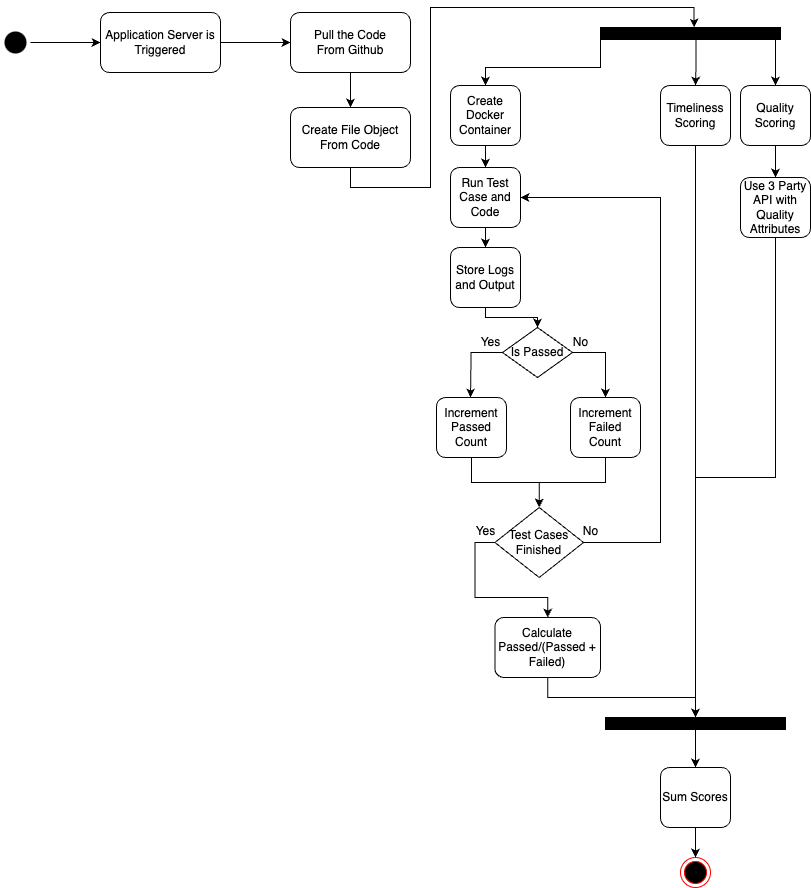
\includegraphics[width=\linewidth]{Images/DD-Sandbox.drawio.png}
    \caption{Submission Scoring}
\end{figure}



